%!TEX root = ../Thesis.tex

\section{Introduction}
\label{sec:introduction1}%

Many engineering applications show nonlinear behaviours, and linear systems cannot provide an acceptable solution in more and more situations. In solid mechanics, such a situation usually occurs when the deformation is large, material response is complex, boundary conditions vary, etc. In this context, linear systems could be seen as approximation of nonlinear systems under limited conditions, e.g., with small deformation.

In general there is no analytical way of finding the solution of a system of nonlinear equations, and this explains why computational sciences have become increasingly in demand.

In the following section we discuss a variation of a problem presented during the course and in the book~\cite{namhokim}.

\section{System of Nonlinear Springs}
\label{sec:system_NL_springs}%

Consider three non-linear springs connected in series and in parallel, as shown in Figure~\ref{fig:springs_first}.

\begin{figure}[H]
    \centering
    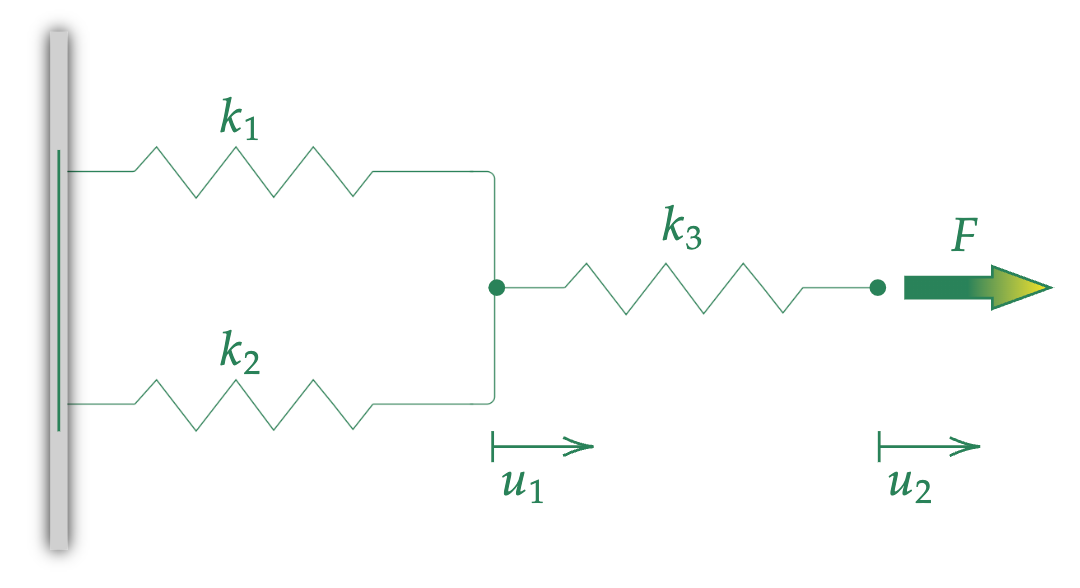
\includegraphics[width=0.8\textwidth]{spring_sys_2.png}
    \caption{System of nonlinear springs.}
    \label{fig:springs_first}
\end{figure}

The stiffness of the springs depends on the elongation of springs such that
\begin{equation*}
\label{eq:spring_1}
k_i = k_i\left( e_i \right) = \alpha_i+\beta_i\cdot e_i\quad [\text{N/mm}],\qquad\qquad i=1,2,3,
\end{equation*}
with $e_i$ being the elongation of the $i$-th spring and coefficients $\left( \alpha_i,\beta_i \right)$ being listed in Table~\ref{table:alpha_beta}. In this way, although the geometry of the problem is linear, it is ruled by nonlinear costitutive laws.

In Figure~\ref{fig:springs_first} is also shown the load application $F=100\ [\text{N}]$ at the tip.

Our interest lies in calculating $u_1$ and $u_2$, the nodal displacements at the two nodes.

\begin{table}[H]
    %\caption*{\textbf{Title of Table (optional)}}
    \centering 
    \begin{tabular}{ccc}
    \hline
    \rowcolor{bluepoli!40} % comment this line to remove the color
    $i$ & $\alpha_i$ & $\beta_i$  \\
    \hline
    1 & 500 & 50 \\
    2 & 200 & 100 \\
    3 & 500 & 100 \\
    \hline
    \end{tabular}
    \\[10pt]
    \caption{Springs coefficients.}
    \label{table:alpha_beta}
\end{table}

From Figure~\ref{fig:main13_1} one can notice that the stiffness (the local tangent) is increasing for increased elongations.

\begin{figure}[H]
    \centering
    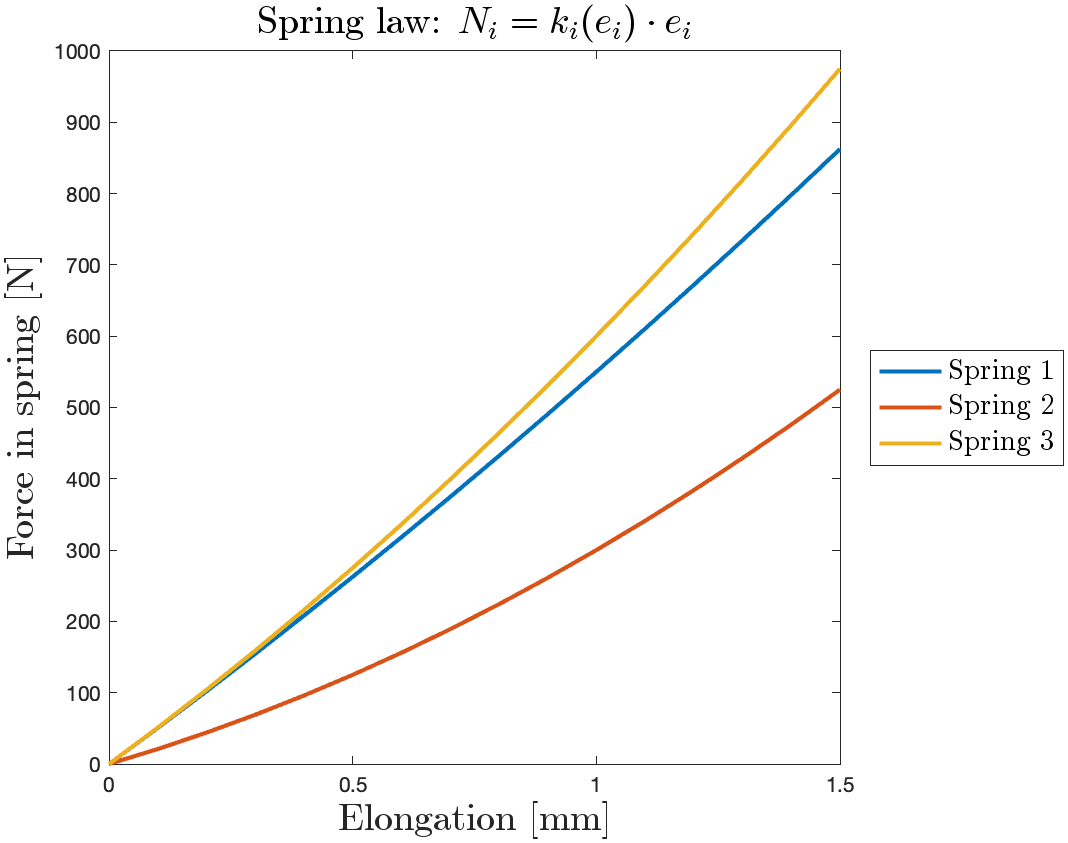
\includegraphics[width=0.9\textwidth]{main13_1.png}
    \caption{Costitutive law plot.}
    \label{fig:main13_1}
\end{figure}

Since springs 1 and 2 are fixed on the wall, their elongation is equivalent to $u_1$, while for spring 3, the elongation is $u_2-u_1$. It's very easy to find out the equilibrium of the two nodes:
\begin{equation*}
\label{eq:spring_2}
\left\{
\begin{aligned}
N_1+N_2-N_3&=0, \\
N_3&=F.\\
\end{aligned}
\right.
\end{equation*}

It follows that the matrix notation of the system in term of unknown displacement $\mathbf{u}$ is
\begin{equation}
\label{eq:spring_25}
\mathbf{P}(\mathbf{u})=\mathbf{f}
\end{equation}
or, in a more physical notation,
\begin{equation*}
\label{eq:spring_275}
\mathbf{F}^{\textbf{int}}(\mathbf{u})=\mathbf{F}^{\textbf{ext}},
\end{equation*}

hence, the system is the following:
\begin{equation*}
\label{eq:spring_3}
\left[
\begin{array}{cc}
 k_1+k_2+k_3 &-k_3 \\
 -k_3 & +k_3
\end{array}
\right]
\left[
\begin{array}{c}
 u_1 \\
 u_2
\end{array}
\right]
=
\left[
\begin{array}{c}
 0 \\
 F
\end{array}
\right].
\end{equation*}

Note that, as we said before, the above equations are not linear as the stiffness matrix contains unknown variables.

Using the given stiffness of springs, the general matrix equation becomes
\begin{equation*}
\label{eq:spring_4}
\begin{cases}
\left( \beta_1+\beta_2-\beta_3 \right)u_1^2 +\left( \alpha_1+\alpha_2+\alpha_3 \right)u_1+2\beta_3u_1u_2-\alpha_3u_2-\beta_3u_2^2=0 \\
\beta_3u_1^2-\alpha_3u_1-2\beta_3u_1u_2+\alpha_3u_2+\beta_3u_2^2=F
\end{cases},
\end{equation*}

which, for the sake of generality, leads to
\begin{equation*}
\label{eq:spring_5}
\begin{cases}
\mathcal{A}u_1^2 +\mathcal{B}u_1+\mathcal{C}u_1u_2+\mathcal{D}u_2+\mathcal{E}u_2^2=0 \\
\mathcal{F}u_1^2 +\mathcal{G}u_1+\mathcal{H}u_1u_2+\mathcal{I}u_2+\mathcal{L}u_2^2=F
\end{cases}.
\end{equation*}

In this way it will be easier to build the system in MATLAB, namely with
\begin{equation}
\label{eq:spring_6}
\left[
\begin{array}{ccccc}
\mathcal{A} & \mathcal{B} & \mathcal{C} & \mathcal{D} & \mathcal{E} \\
\mathcal{F} & \mathcal{G} & \mathcal{H} & \mathcal{I} & \mathcal{L}
\end{array}
\right]
\left[
\begin{array}{c}
u_1^2 \\
u_1 \\
u_1u_2 \\
u_2 \\
u_2^2
\end{array}
\right].
\end{equation}

Finally, the assembled system is
\begin{equation*}
\label{eq:spring_7}
\begin{cases}
50u_1^2+1200u_1+200u_1u_2-500u_2-100u_2^2=0 \\
100u_1^2-500u_1-200u_1u_2+500u_2+100u_2^2=100
\end{cases}.
\end{equation*}

In the following section, a method of solving the system of nonlinear equations is discussed.

\section{Numerical Solution}
\label{sec:numerical_solution1}%

Before discussing systems, it is important to understand the problem of numerical approximation of the zeros of a real-valued function of one variable, that is
\begin{equation*}
\label{eq:spring_8}
\boxed{\text{Given }f:(a,b)\to\mathbb{R},\text{ find }\alpha\in\mathbb{R}\text{ s.t. }f(\alpha)=0}
\end{equation*}

There are several iterative methods to solve this rootfinding problem, such as the bisection method, the chord method, the secant method, fixed point methods, etc. For a more complete treatment of these, see for example \cite{quarter}.

In the following we analyze another algorithm: the Newton's method, also known as the \textbf{Newton–Raphson method}.

Assuming that $f\in\mathcal{C}^1\big( (a,b) \big)$ and that $\alpha$ is a simple root of $f$, if we let
\begin{equation*}
\label{eq:spring_9}
q_k=f' ( x^k ),\qquad\forall k\geq 0
\end{equation*}
and assign the initial value $x^0$, we obtain the Newton scheme
\begin{equation}
\label{eq:spring_10}
x^{k+1}=x^k-\frac{f( x^k )}{q_k},\qquad k\geq 0.
\end{equation}

The idea is clarified by looking at the first-order series expansion of $f(x)$ in the neighborhood of $x^k$
\begin{equation*}
\label{eq:spring_11}
f(x)\approx f ( x^k )+\left[\frac{\text{d}f}{\text{d}x}(x^k)\right](x-x^k) \qquad\ \xrightarrow[]{x=x^{k+1}} \qquad \text{Eq.~\eqref{eq:spring_10}}
\end{equation*}

and by Figure~\ref{fig:quart1}.

\begin{figure}[H]
    \centering
    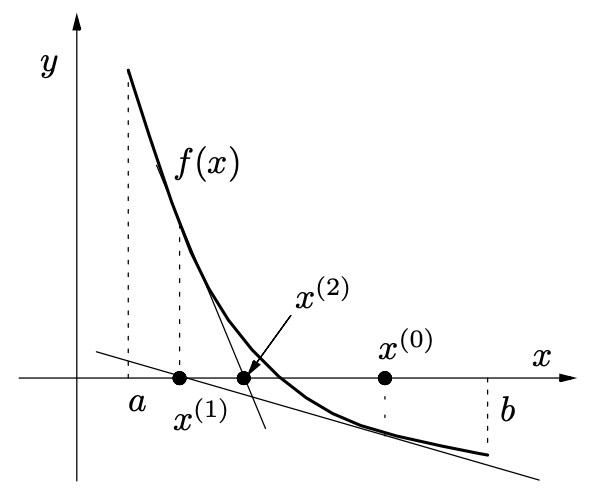
\includegraphics[width=0.5\textwidth]{quart1.png}
    \caption{Geometric approach of Newton-Raphson method: first two steps.}
    \label{fig:quart1}
\end{figure}

This method has an high convergence order, namely $p=2$, i.e.
\begin{equation}
\label{eq:spring_12}
\exists C>0\qquad\text{s.t.}\qquad \lim_{k\to\infty}\frac{\left| x^{k+1}-\alpha \right|}{\left| x^{k}-\alpha \right|^2}=C,
\end{equation}
but $\alpha$ should be a simple root and the initial value $x^0$ should be \emph{close} to the solution, because the method does not always guarantee convergence (actually, sometimes the solution may diverge or oscillate between two points). 

An immediate extension of Newton-Raphson’s method~\eqref{eq:spring_10} for the nonlinear system~\eqref{eq:spring_25} can be recursively formulated as
\begin{equation*}
\label{eq:spring_13}
\mathbf{u}^{k+1}=\mathbf{u}^k+\frac{ \mathbf{f}-\mathbf{P}(\mathbf{u}^k) }{\mathbf{K}_T^k}\qquad \text{with}\qquad \mathbf{K}_T^k=\frac{\partial\mathbf{P}}{\partial\mathbf{u}}(\mathbf{u}^k) ,
\end{equation*}

which leads to the following algorithm:
\begin{subequations}
\label{eq:spring_14}
\begin{align}
\text{given }\mathbf{u}^0,\text{ for }k=&0,1,\dots,\text{ until convergence:} \nonumber \\
\text{compute}\qquad&\mathbf{K}_T^k\text{ and } \mathbf{R}^k=\mathbf{f}-\mathbf{P}(\mathbf{u}^k) , \label{eq:spring_15} \\
\text{solve}\qquad &\mathbf{K}_T^k\,\Delta\mathbf{u}^k=\mathbf{R}^k , \label{eq:spring_16} \\
\text{set}\qquad&\mathbf{u}^{k+1}=\mathbf{u}^k+\Delta\mathbf{u}^k. \label{eq:spring_17}
\end{align}
\end{subequations}

In general, this solution will not satisfy the system of nonlinear equations exactly and there will be some residual (or unbalance force in a physical point of view). If the $k$-th residual is smaller than a given tolerance, the solution $\mathbf{u}^{k+1}$ can be accepted as the accurate solution, and the process stops. The stopping criterion is expressed as follows
\begin{equation}
\label{eq:spring_18}
\text{conv}^{\,k+1}=\frac{\displaystyle\sum_{j=1}^n\left( \text{R}_j^{k+1} \right)^2}{1+\displaystyle\sum_{j=1}^n\left( \text{f}_j \right)^2},
\end{equation}
and, in order to show quadratic convergence as in Eq.~\eqref{eq:spring_12}, it is often enough to show that $\textbf{conv}$ reduces quadratically at each iteration.

\smallskip

\begin{marker}
From Eq.~\eqref{eq:spring_16}, one can notice that at each step $k$ the solution of a linear system with matrix $\mathbf{K}_T^k$ is required, thus the matrix cannot be singular. We will use the \emph{backslash} MATLAB command to solve the system, but the computational cost increases as $n^2$. There are several ways to solve this, for example use the LU decomposition and keep it fixed for some iterations, or just keep $\mathbf{K}_T^k$ fixed. See Secion~\ref{sec:MATLAB_implementation1} for further details.
\end{marker}

\newpage

\section{MATLAB Implementation}
\label{sec:MATLAB_implementation1}%

Here we present and explain the MATLAB scripts used to solve the problem. Algorithms are listed in the Subsection~\ref{sub:matlab_scripts1}.

In \texttt{main11} (Algorithm~\ref{alg:main11}) we implement the Newton-Raphson method previously described. Here two auxiliary functions are used to compute the internal force vector $\mathbf{P}(\mathbf{u})$ and its Jacobian matrix $\mathbf{K}_T$ at each iteration. These MATLAB functions \newline
\texttt{generate\_int\_force} (Algorithm~\ref{alg:generate_int_force}) and \texttt{generate\_jacobian} (Algorithm~\ref{alg:generate_jacobian}) are merely based on Eq.~\eqref{eq:spring_6}.

The output of the code is the following:
\begin{matlaboutput}
*********************************************************************
RESULTS
*********************************************************************

iter   u1        u2        conv
   0   2.00000   2.00000   4.00960e+02
   1   0.53846   0.73846   1.00124e+01
   2   0.16655   0.35914   4.30187e-02
   3   0.13889   0.33147   1.31776e-06
   4   0.13873   0.33132   1.29140e-15

Convergence reached in 4 iterations

*********************************************************************
\end{matlaboutput}

The initial guess choosen was $\mathbf{u}^0=[2;2]$, but we can easily repeat the process for other initial estimates. For example, with $\mathbf{u}^0=[0;0]$ we have 
\begin{matlaboutput}
*********************************************************************
RESULTS
*********************************************************************

iter   u1        u2        conv
   0   0.00000   0.00000   9.99900e-01
   1   0.14286   0.34286   1.68796e-03
   2   0.13874   0.33133   3.87449e-09
   3   0.13873   0.33132   1.81925e-20

Convergence reached in 3 iterations

*********************************************************************
\end{matlaboutput}

\newpage

and with $\mathbf{u}^0=[9;9]$ we have
\begin{matlaboutput}
*********************************************************************
RESULTS
*********************************************************************

iter   u1        u2        conv
   0   9.00000   9.00000   3.40378e+04
   1   3.60294   3.80294   1.90534e+03
   2   1.14953   1.34212   8.15108e+01
   3   0.28541   0.47799   1.25440e+00
   4   0.14284   0.33542   9.29483e-04
   5   0.13874   0.33132   6.38409e-10

Convergence reached in 5 iterations

*********************************************************************
\end{matlaboutput}

From all these outputs we can say that as MATLAB program iterates, the displacements converges to the numerical solution $\mathbf{u}=[0.13873;0.33132]$ mm; secondly, the number of iterations depends on the starting point, however the residual reduction via convergence criterion~\eqref{eq:spring_18} is approximately quadratic.

We can double check the accuracy of our solution via plotting the surfaces of the system of nonlinear equations with zero-level contour. The results we obtain with \texttt{main12} (Algorithm~\ref{alg:main12}) ant the \texttt{plotzeros} function (Algorithm~\ref{alg:plotzeros}) are the following figures:
\begin{figure}[H]
    \centering
    \subfloat[Zero-level contour plot.\label{fig:main12_1}]{
        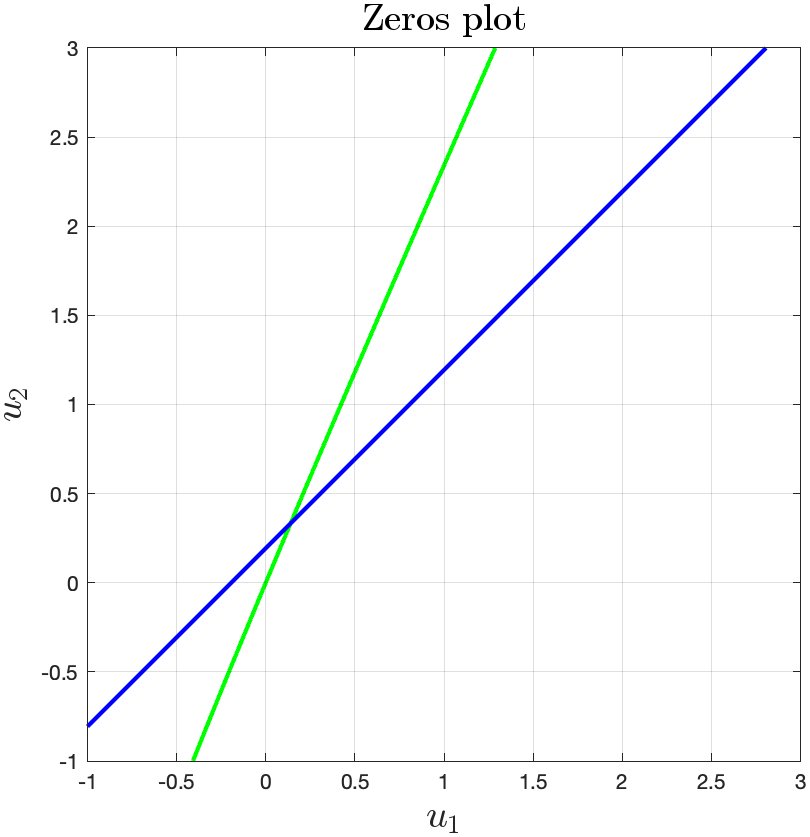
\includegraphics[scale=0.4]{Images/main12_1.png}
    }
    \quad
    \subfloat[3D Surface plot.\label{fig:main12_2}]{
        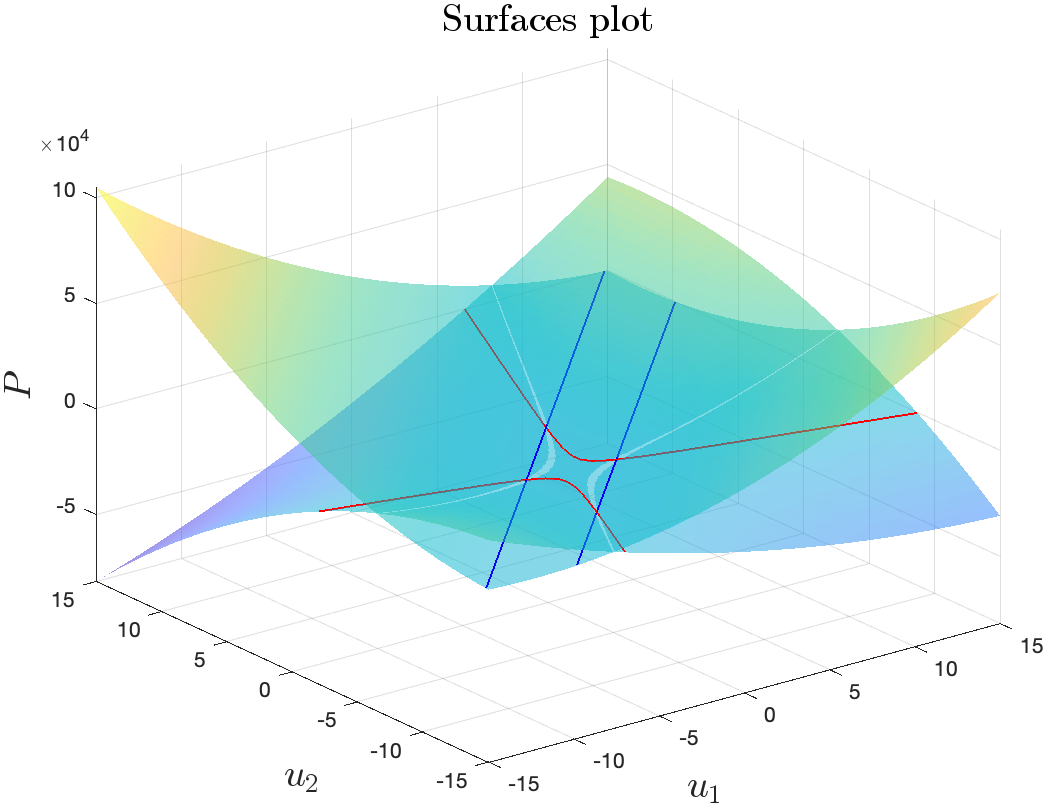
\includegraphics[scale=0.4]{Images/main12_2.png}
    }
    \caption{Zero-level contour and Surface plots.}
    \label{fig:main12}
\end{figure}

Note that there exist four solutions to the problem, but only one of them, the one we found, is positive.

\newpage

Thanks to script \texttt{main13} (Algorithm~\ref{alg:main13}) we generate useful data for the subsequent processing in Abaqus (see Section~\ref{sec:abaqus_implementation1}) and Figure~\ref{fig:main13_1}.

\vspace{5mm}

The Newton–Raphson method requires that at each iteration, the Jacobian matrix should be formed and the system of linearized equations should be solved for the increment of the solution. Computationally, these are expensive tasks. The \textbf{Modified Newton–Raphson method} is an attempt to make these procedures less expensive. Instead of formulating a new tangent stiffness matrix at each iteration, the initial tangent stiffness matrix is repeatedly used for all iterations. 

Through \texttt{main14} (Algorithm~\ref{alg:main14}) we implement the Modified Newton-Raphson method, gaining the following output:
\begin{matlaboutput}
*********************************************************************
RESULTS
*********************************************************************

iter   u1        u2        conv
   0   2.00000   2.00000   4.00960e+02
   1   0.53846   0.73846   1.00124e+01
   2   0.29199   0.48399   1.38037e+00
   3   0.20185   0.39448   2.24486e-01
   4   0.16538   0.35796   3.94896e-02
   5   0.15010   0.34268   7.13582e-03
   6   0.14360   0.33618   1.30509e-03
   7   0.14082   0.33340   2.39875e-04
   8   0.13963   0.33221   4.41837e-05
   9   0.13912   0.33170   8.14585e-06
  10   0.13890   0.33148   1.50238e-06
  11   0.13880   0.33139   2.77140e-07
  12   0.13876   0.33135   5.11268e-08
  13   0.13875   0.33133   9.43218e-09
  14   0.13874   0.33132   1.74013e-09
  15   0.13874   0.33132   3.21035e-10

Convergence reached in 15 iterations

*********************************************************************
\end{matlaboutput}

The method usually requires a greater number of iterations for convergence than that of the regular Newton–Raphson method. However, the overall computational cost to obtain the solution can be made less because each iteration is much faster than that of the regular Newton–Raphson method. The method is also a little more stable and is not prone to divergence.

\newpage

\subsection{MATLAB scripts}
\label{sub:matlab_scripts1}%

\begin{matlab}{main11}{alg:main11}
clear; clc; close;
% data
tol = 1.0e-9; iter = 0; max_iter = 100; u = [2;2]; old_u = u; F = 100;
a1 = 500; b1 = 50; a2 = 200; b2 = 100; a3 = 500; b3 = 100;
k1 = a1+b1*u(1); k2 = a2+b2*u(1); k3 = a3+b3*(u(2)-u(1));
% internal force vector
P = generate_int_force(u,a1,b1,a2,b2,a3,b3);
% external force vector
FF = [0; F];
% residual
R = FF - P;
% convergence parameter
conv = (R(1)^2+R(2)^2)/(1+FF(1)^2+FF(2)^2);
conv_rate = [];
fprintf('%s', repmat('*', 1, 69));
fprintf('\nRESULTS\n');
fprintf('%s', repmat('*', 1, 69));
fprintf('\n');
fprintf('\niter   u1        u2        conv');
fprintf('\n %3d   %7.5f   %7.5f   %7.5e',iter,u(1),u(2),conv);
while conv > tol && iter < max_iter
    % jacobian matrix of P
    Kt = generate_jacobian(u,a1,b1,a2,b2,a3,b3);
    % check if it is singular
    if det(Kt)==0
        fprintf('\n\n');
        error('Jacobian is singular!')
    end
    % solve the linear system
    delta_u = Kt\R;
    % update of the solution
    u = old_u + delta_u;
    % update of the internal force vector
    P = generate_int_force(u,a1,b1,a2,b2,a3,b3);
    % update of the residual
    R = FF - P;
    % update of the convergence parameter
    conv = (R(1)^2+R(2)^2)/(1+FF(1)^2+FF(2)^2);
    % save it in a vector
    conv_rate = [conv_rate; conv];
    % ready for a new iteration
    old_u = u;


    iter = iter + 1;
    % print of the results
    fprintf('\n %3d   %7.5f   %7.5f   %7.5e',iter,u(1),u(2),conv);
end
if iter==max_iter
    fprintf('\n\n');
    error('Convergence not reached!')
end
fprintf('\n\nConvergence reached in %d iterations',iter); 
fprintf('\n\n');
fprintf('%s', repmat('*', 1, 69)); fprintf('\n\n');
% p = log2(conv_rate(1:end-1)./conv_rate(2:end));

\end{matlab}

\bigskip

\begin{matlab}{generate int force}{alg:generate_int_force}
function P = generate_int_force(u,a1,b1,a2,b2,a3,b3)
A = b1+b2-b3; B = a1+a2+a3; C = 2*b3; D = -a3; E = -b3;
F = b3; G = -a3; H = -2*b3; I = a3; L = b3;
U = [u(1)^2;u(1);u(1)*u(2);u(2);u(2)^2];
P1 = [A,B,C,D,E;F,G,H,I,L];
P = P1*U;
end
\end{matlab}

\bigskip

\begin{matlab}{generate jacobian}{alg:generate_jacobian}
function J = generate_jacobian(u,a1,b1,a2,b2,a3,b3)
A = b1+b2-b3; B = a1+a2+a3; C = 2*b3; D = -a3; E = -b3;
F = b3; G = -a3; H = -2*b3; I = a3; L = b3;
U = [u(1);u(2);1];
J1 = [2*A,C,B;C,2*E,D;2*F,H,G;H,2*L,I];
J2 = J1*U;
J = [J2(1),J2(2);J2(3),J2(4)];
end
\end{matlab}

\newpage

\begin{matlab}{main12}{alg:main12}
clear; clc; close;
a1 = 500; b1 = 50; a2 = 200; b2 = 100; a3 = 500; b3 = 100; f = 100;
A = b1+b2-b3; B = a1+a2+a3; C = 2*b3; D = -a3; E = -b3;
F = b3; G = -a3; H = -2*b3; I = a3; L = b3;
fun = @(u) [A*u(1)^2+B*u(1)+C*u(1)*u(2)+D*u(2)+E*u(2)^2;
            F*u(1)^2+G*u(1)+H*u(1)*u(2)+I*u(2)+L*u(2)^2-f];
plotzeros(fun, [-1 3], [-1 3])
%
figure()
[X,Y] = meshgrid(-15:.5:15);
Z1 = (b1+b2-b3)*X.^2+(a1+a2+a3)*X+2*b3*X.*Y-a3*Y-b3*Y.^2;
s1 = surf(X,Y,Z1,'FaceAlpha',0.5);
s1.EdgeColor = 'none';
xlabel('$u_1$','Interpreter','latex',FontSize=18)
ylabel('$u_2$','Interpreter','latex',FontSize=18)
zlabel('$P$','Interpreter','latex',FontSize=18)
title('Surfaces plot','Interpreter','latex',FontSize=18)
hold on
Z2 = b3*X.^2-a3*X-2*b3*X.*Y+a3*Y+b3*Y.^2-F;
s2 = surf(X,Y,Z2,'FaceAlpha',0.5);
s2.EdgeColor = 'none';
contour(X,Y,Z1, [0 0], 'r', 'LineWidth', 1);
contour(X,Y,Z2, [0 0], 'b', 'LineWidth', 1);
\end{matlab}

\bigskip

\begin{matlab}{plotzeros}{alg:plotzeros}
function plotzeros(fun, x_limits, y_limits, varargin)
if nargin > 3
    sample_len = varargin{1};
else
    sample_len = 500;
end
v_dis_x = linspace(x_limits(1), x_limits(2), sample_len);
v_dis_y = linspace(y_limits(1), y_limits(2), sample_len);
n_dis_x = length(v_dis_x);
n_dis_y = length(v_dis_y);
Z_1 = zeros(n_dis_y, n_dis_x);
Z_2 = zeros(n_dis_y, n_dis_x);
for i = 1:n_dis_x
    for j = 1:n_dis_y
        funz = fun([v_dis_x(i); v_dis_y(j)]); 
        Z_1(j,i) = funz(1); Z_2(j,i) = funz(2);
    end
end


contour(v_dis_x, v_dis_y, Z_1, [0 0], 'Linecolor',[0 1 0], 'Linewidth', 2)
hold on
contour(v_dis_x, v_dis_y, Z_2, [0 0], 'Linecolor',[0 0 1], 'Linewidth', 2)
axis equal
grid on
xlabel('$u_1$','Interpreter','latex',FontSize=18)
ylabel('$u_2$','Interpreter','latex',FontSize=18)
title('Zeros plot','Interpreter','latex',FontSize=18)
end
\end{matlab}

\bigskip

\begin{matlab}{main13}{alg:main13}
clear; clc; close; format shorte
U = 0:0.1:1.5; Ut = U'
a1 = 500; b1 = 50; a2 = 200; b2 = 100; a3 = 500; b3 = 100;
k1 = a1+b1*Ut; k2 = a2+b2*Ut; k3 = a3+b3*Ut; kEQ = k1+k2;
F1 = k1.*Ut;
figure(1)
plot(Ut,F1,'linewidth',2)
xlabel('Elongation [mm]','Interpreter','latex',FontSize=18)
ylabel('Force in spring [N]','Interpreter','latex',FontSize=18)
title('Spring law: $N_i=k_i(e_i)\cdot e_i$','Interpreter','latex',FontSize=18)
hold on
F2 = k2.*Ut;
plot(Ut,F2,'linewidth',2)
F3 = k3.*Ut;
plot(Ut,F3,'linewidth',2)
legend('Spring 1','Spring 2','Spring 3','Interpreter','latex',Location='eastoutside',FontSize=14)
F12 = kEQ.*Ut
figure(2)
plot(Ut,F12,'linewidth',2)
xlabel('Elongation [mm]','Interpreter','latex',FontSize=18)
ylabel('Force in spring [N]','Interpreter','latex',FontSize=18)
title('Spring law: $N_i=k_i(e_i)\cdot e_i$','Interpreter','latex',FontSize=18)
hold on
F3 = k3.*Ut
plot(Ut,F3,'linewidth',2)
legend('Spring 1+2','Spring 3','Interpreter','latex',Location='eastoutside',FontSize=14)
\end{matlab}

\newpage

\begin{matlab}{main14}{alg:main14}
clear; clc; close;
tol = 1.0e-9; iter = 0; max_iter = 100; u = [2;2]; old_u = u; F = 100;
a1 = 500; b1 = 50; a2 = 200; b2 = 100; a3 = 500; b3 = 100;
k1 = a1+b1*u(1); k2 = a2+b2*u(1); k3 = a3+b3*(u(2)-u(1));
P = generate_int_force(u,a1,b1,a2,b2,a3,b3);
% jacobian matrix of P: FIXED
Kt = generate_jacobian(u,a1,b1,a2,b2,a3,b3);
FF = [0; F];
R = FF - P;
conv = (R(1)^2+R(2)^2)/(1+FF(1)^2+FF(2)^2);
conv_rate = [];
fprintf('%s', repmat('*', 1, 69));
fprintf('\nRESULTS\n');
fprintf('%s', repmat('*', 1, 69));
fprintf('\n');
fprintf('\niter   u1        u2        conv');
fprintf('\n %3d   %7.5f   %7.5f   %7.5e',iter,u(1),u(2),conv);
while conv > tol && iter < max_iter
    delta_u = Kt\R;
    u = old_u + delta_u;
    P = generate_int_force(u,a1,b1,a2,b2,a3,b3);
    R = FF - P;
    conv = (R(1)^2+R(2)^2)/(1+FF(1)^2+FF(2)^2);
    conv_rate = [conv_rate; conv];
    old_u = u;
    iter = iter + 1;
    fprintf('\n %3d   %7.5f   %7.5f   %7.5e',iter,u(1),u(2),conv);
end
if iter==max_iter
    fprintf('\n\n');
    error('Convergence not reached!')
end
fprintf('\n\nConvergence reached in %d iterations',iter); 
fprintf('\n\n');
fprintf('%s', repmat('*', 1, 69)); fprintf('\n\n');
% p = log2(conv_rate(1:end-1)./conv_rate(2:end));
\end{matlab}

\newpage

\section{Abaqus Implementation}
\label{sec:abaqus_implementation1}%

Here we solve the problem through the Abaqus Software by using spring-like connectors. The adopted units of measure are mm and N in order to be consistent, as Abaqus requires.

Before starting, let's remark that our nonlinear system shown in Figure~\ref{fig:springs_first} can be semplified in a system of two serial connected springs:
\begin{figure}[H]
    \centering
    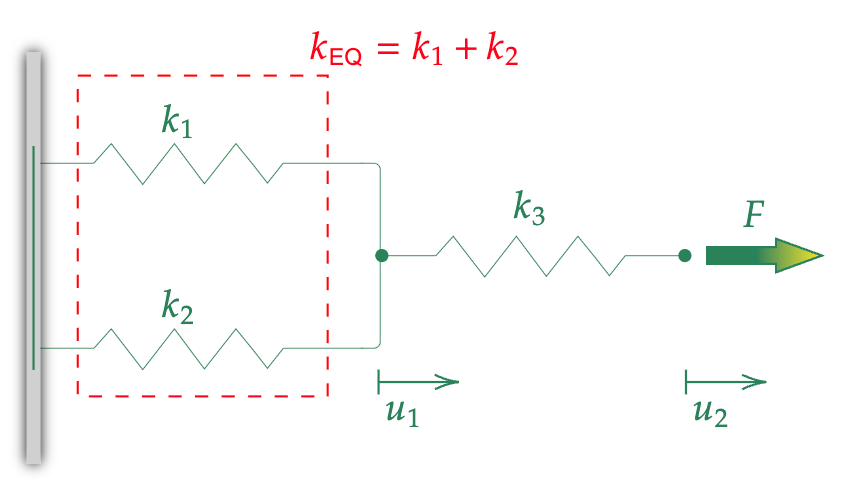
\includegraphics[width=0.5\textwidth]{spring_sys_3.png}
    \caption{Equivalent system of nonlinear springs.}
    \label{fig:springs_second}
\end{figure}

\subsection{Interaction module}
\label{interaction_module1}%

We define the nodes of the spring system by setting three colinear reference points (the distance between the nodes is not important) using the "Create Reference Point" button. Then we re-scale the view and the result is shown in Figure~\ref{fig:a2}.
\begin{figure}[H]
    \centering
    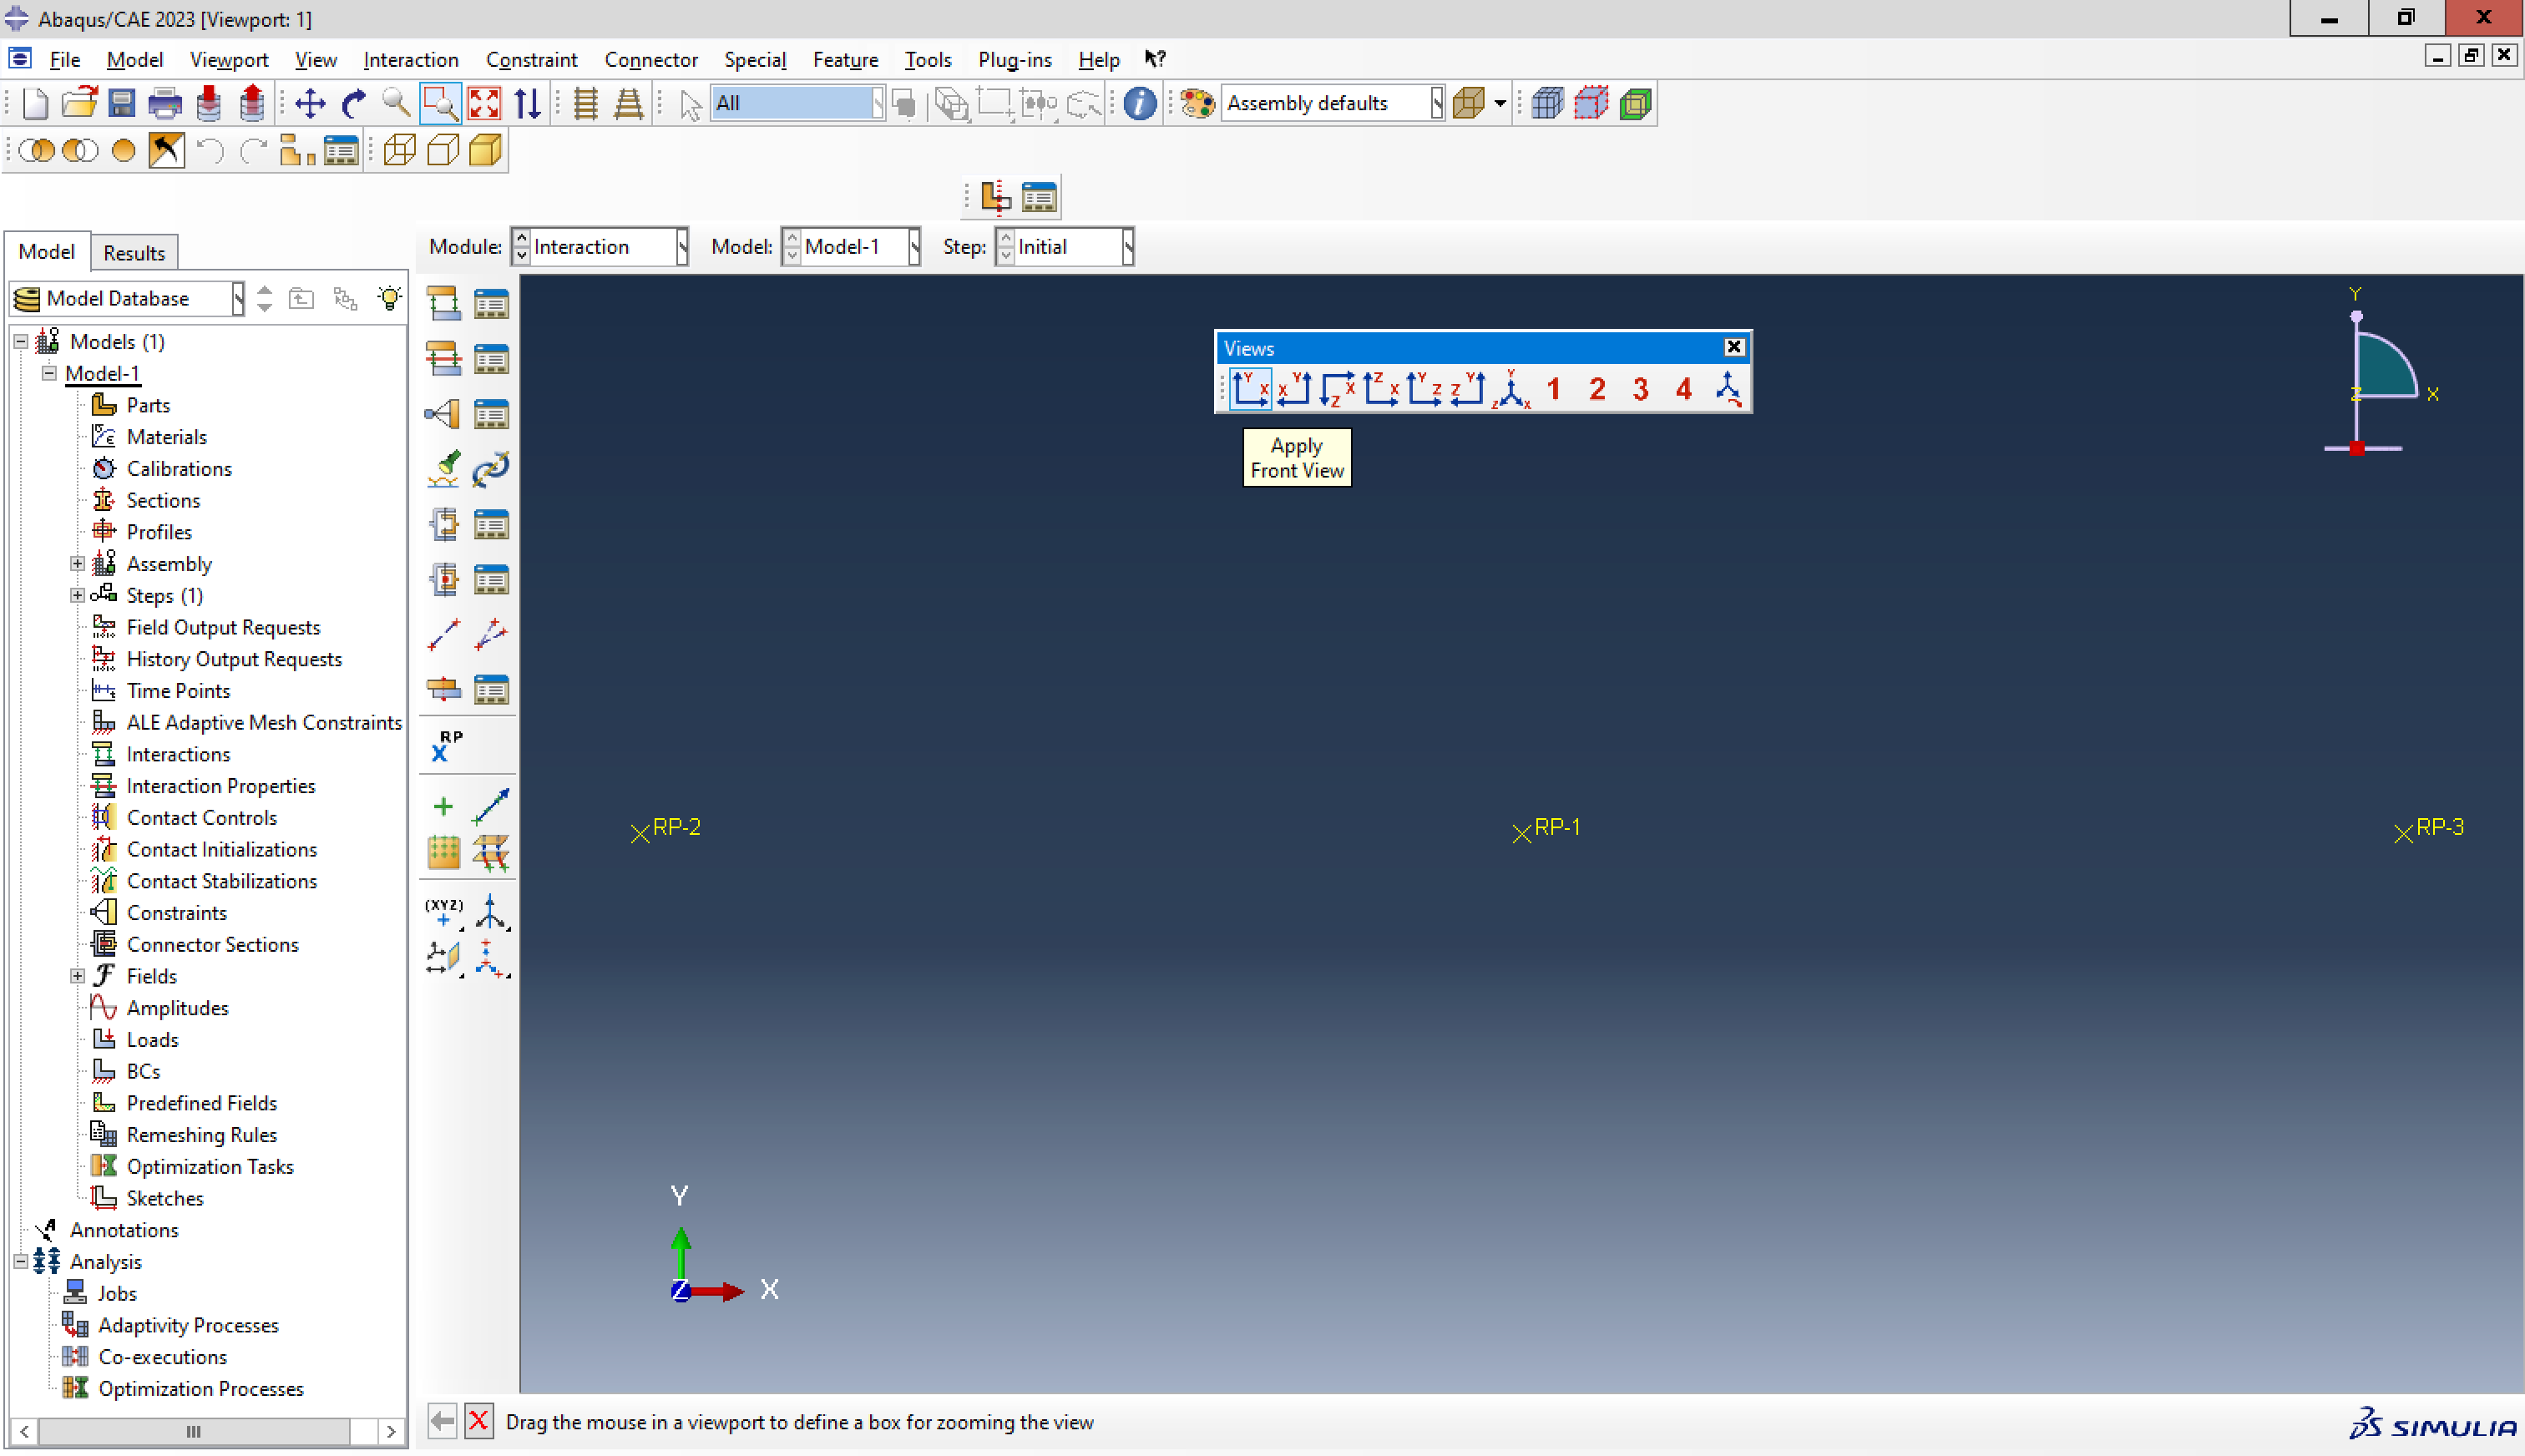
\includegraphics[width=0.9\textwidth]{Images/ab1/a2.png}
    \caption{Reference points.}
    \label{fig:a2}
\end{figure}

\newpage

We proceed by creating the wire feature by clicking on the "Create Wire Feature" 
\begin{figure}[H]
    \centering
    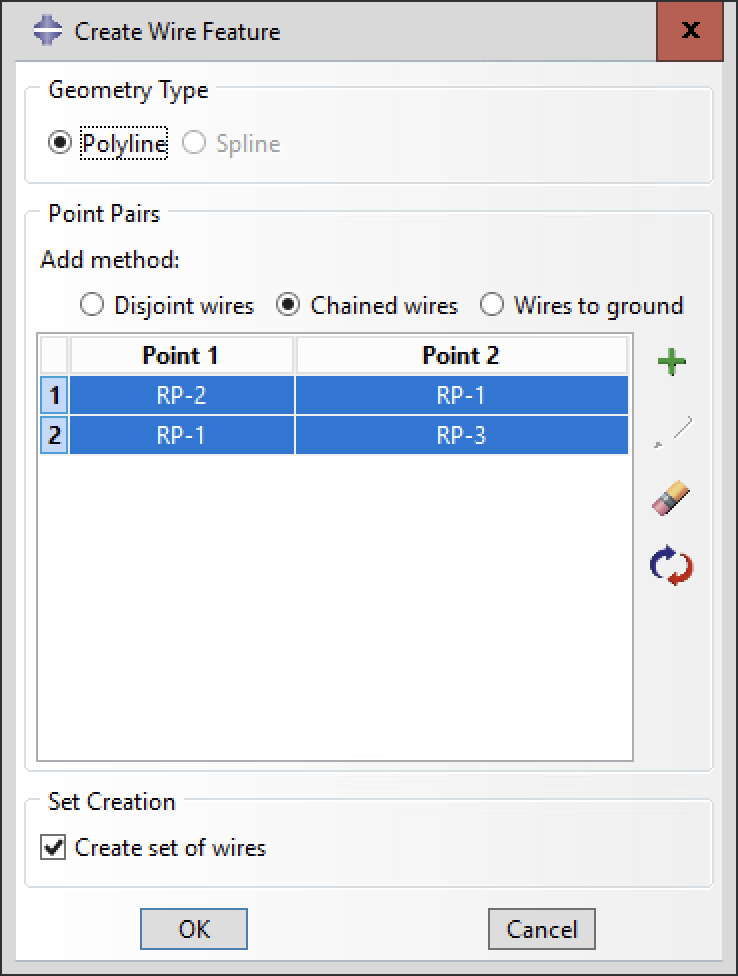
\includegraphics[width=0.4\textwidth]{Images/ab1/a4.png}
    \caption{Wire features.}
    \label{fig:a4}
\end{figure}

and the result is the following:
\begin{figure}[H]
    \centering
    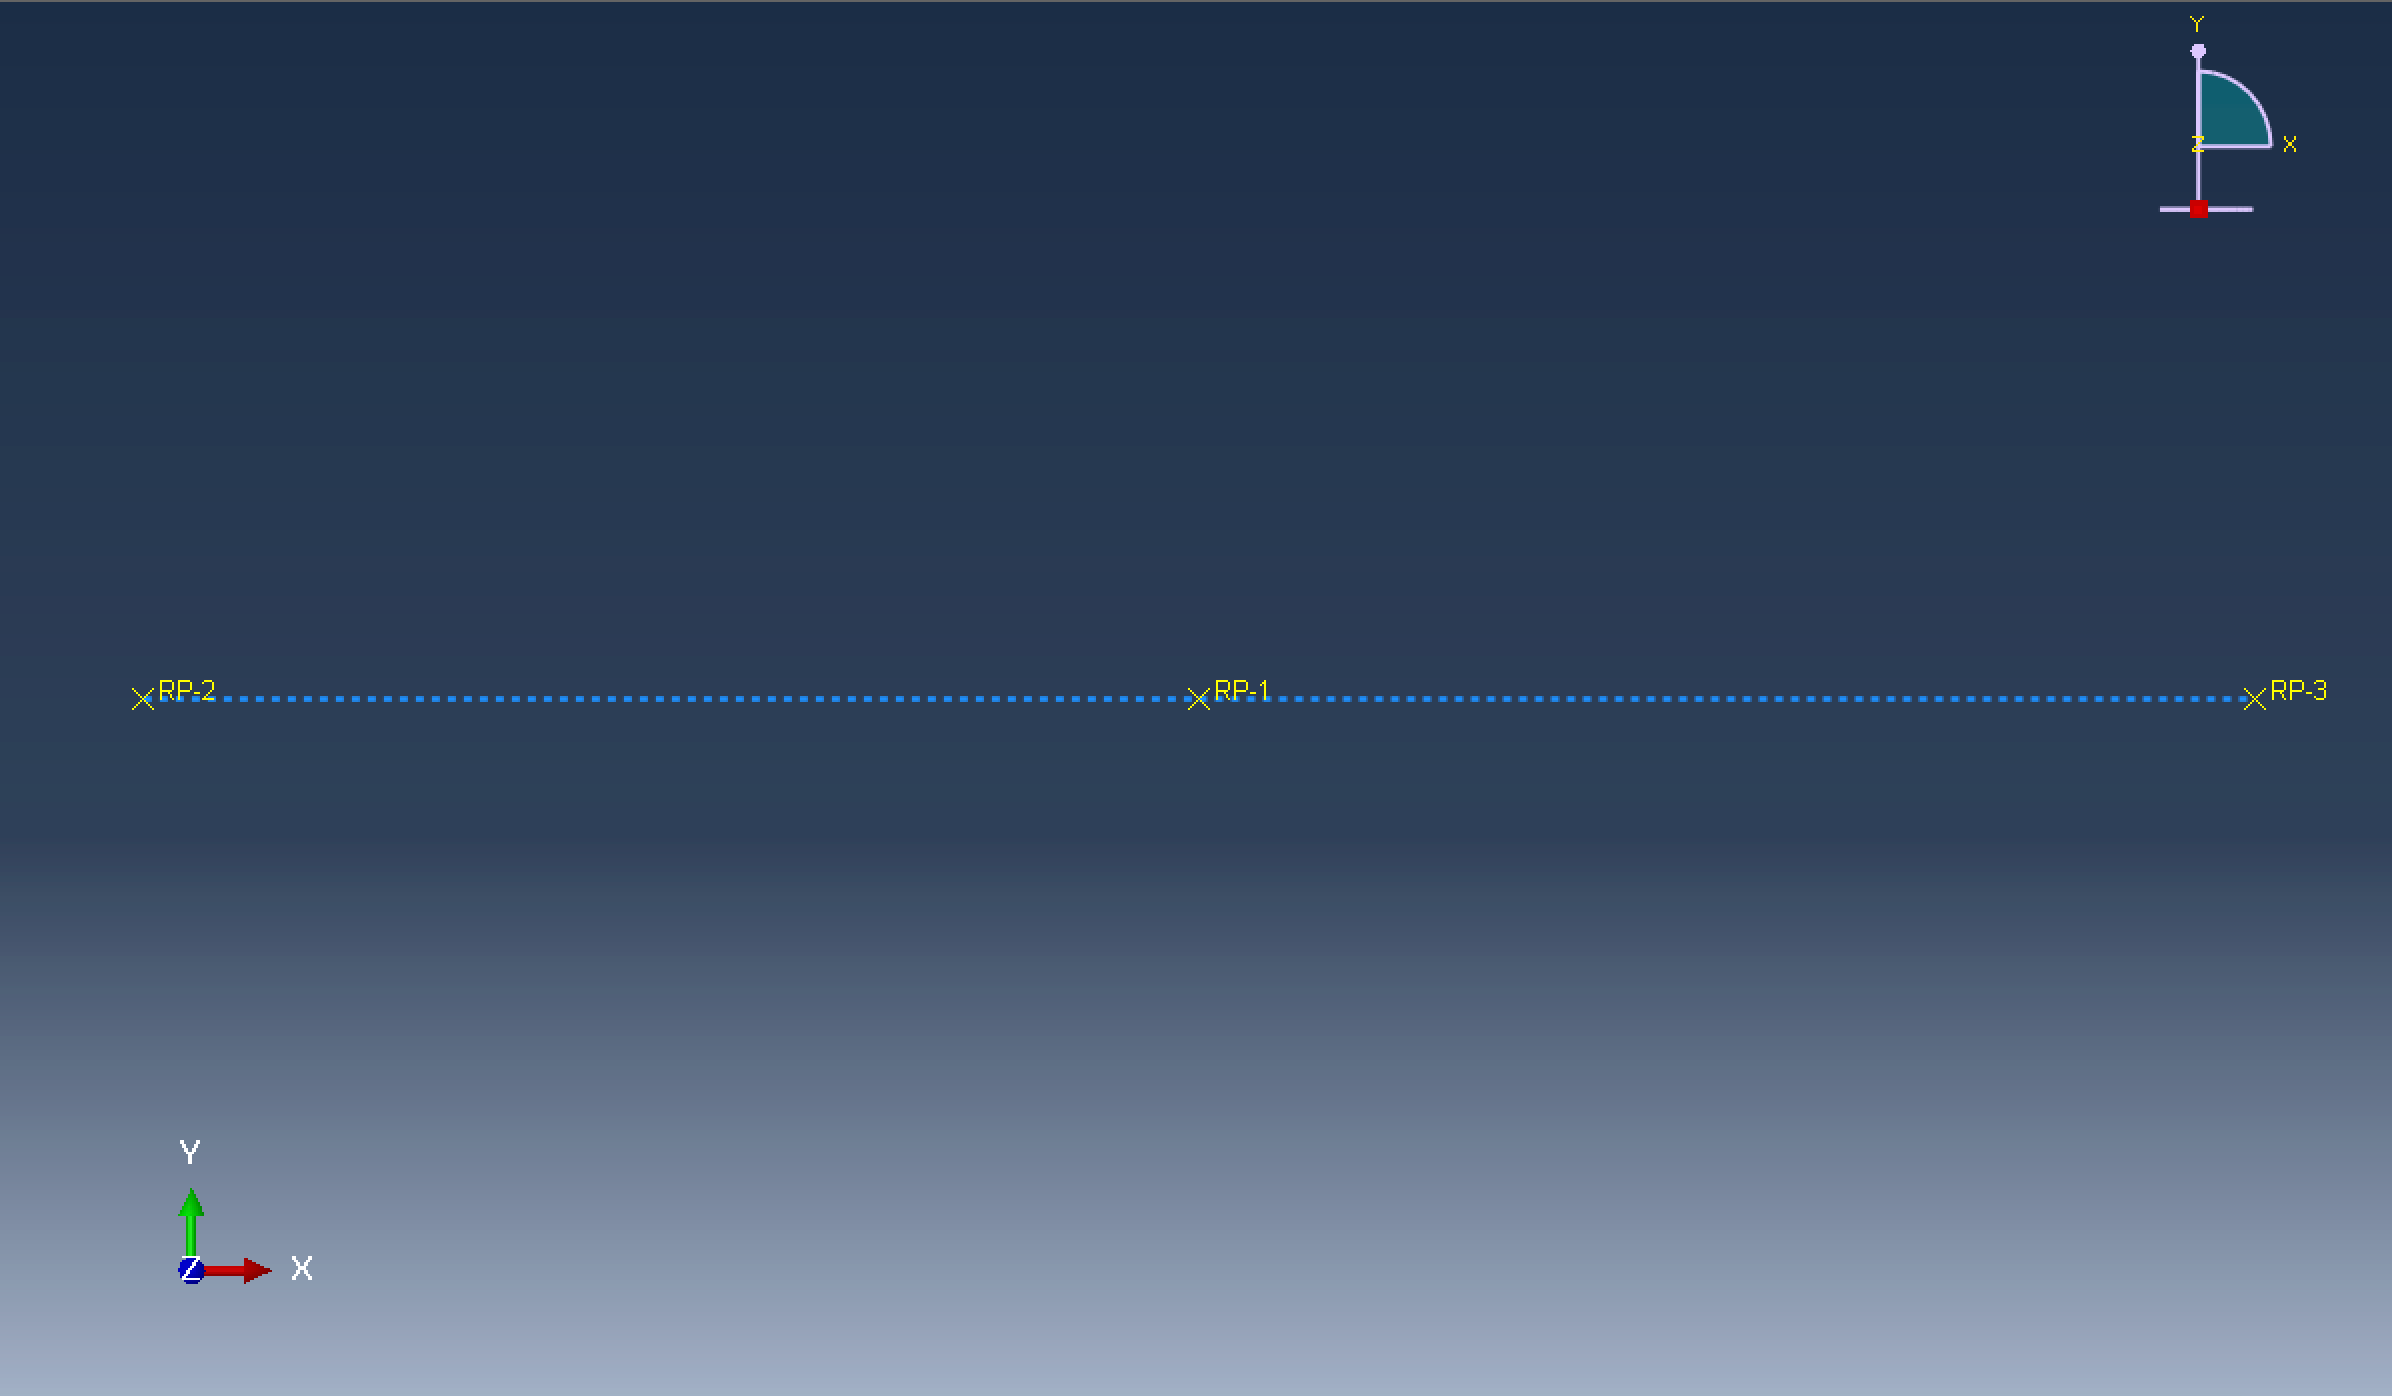
\includegraphics[width=0.9\textwidth]{Images/ab1/a5.png}
    \caption{Middle result of Interaction module.}
    \label{fig:a5}
\end{figure}

\newpage

A new \emph{section} should be defined for each springs. In the "Connector Section Manager", for both springs, we set the connection category as basic and the connection translational type as axial:
\begin{figure}[H]
    \centering
    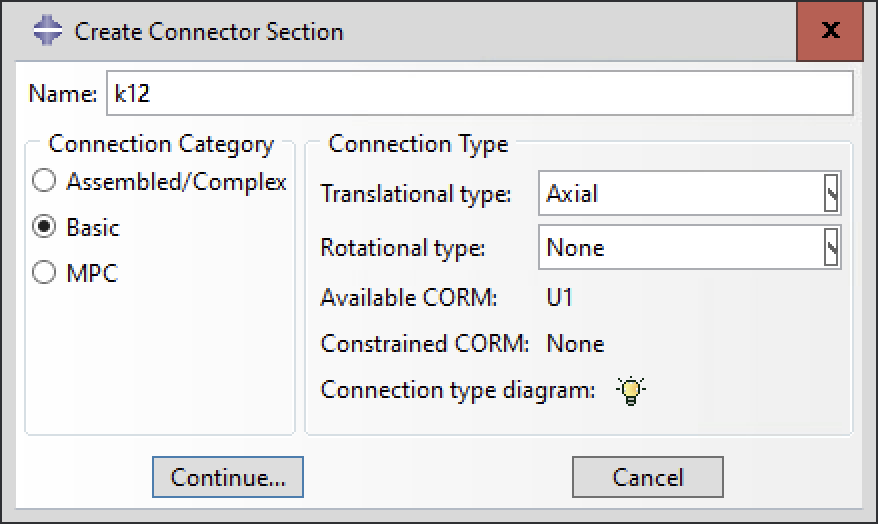
\includegraphics[width=0.4\textwidth]{Images/ab1/a7.png}
    \caption{Connector Section features.}
    \label{fig:a7}
\end{figure}

Here we manage to introduce nonlinearity by pasting the tables of values obtained with Algorithm~\ref{alg:main13} in MATLAB:
\begin{figure}[H]
    \centering
    \subfloat[Behavior options of Spring 1+2.\label{fig:a8}]{
        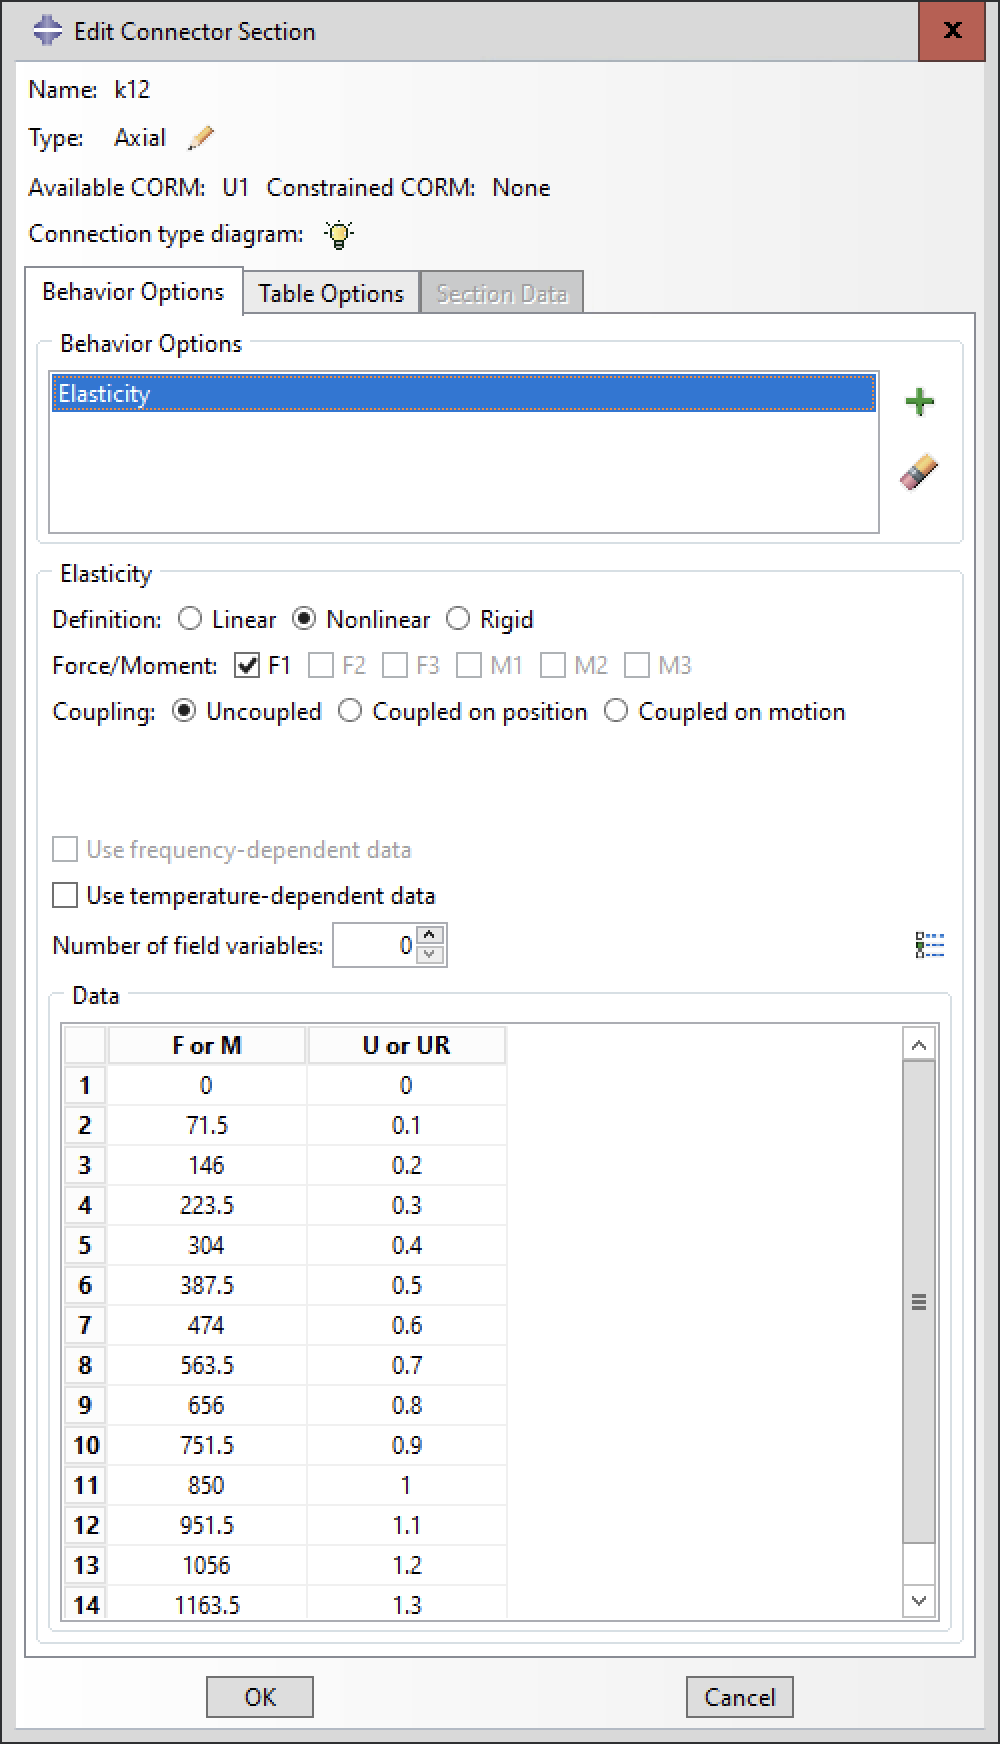
\includegraphics[scale=0.4]{Images/ab1/a8.png}
    }
    \quad
    \subfloat[Behavior options of Spring 3.\label{fig:a9}]{
        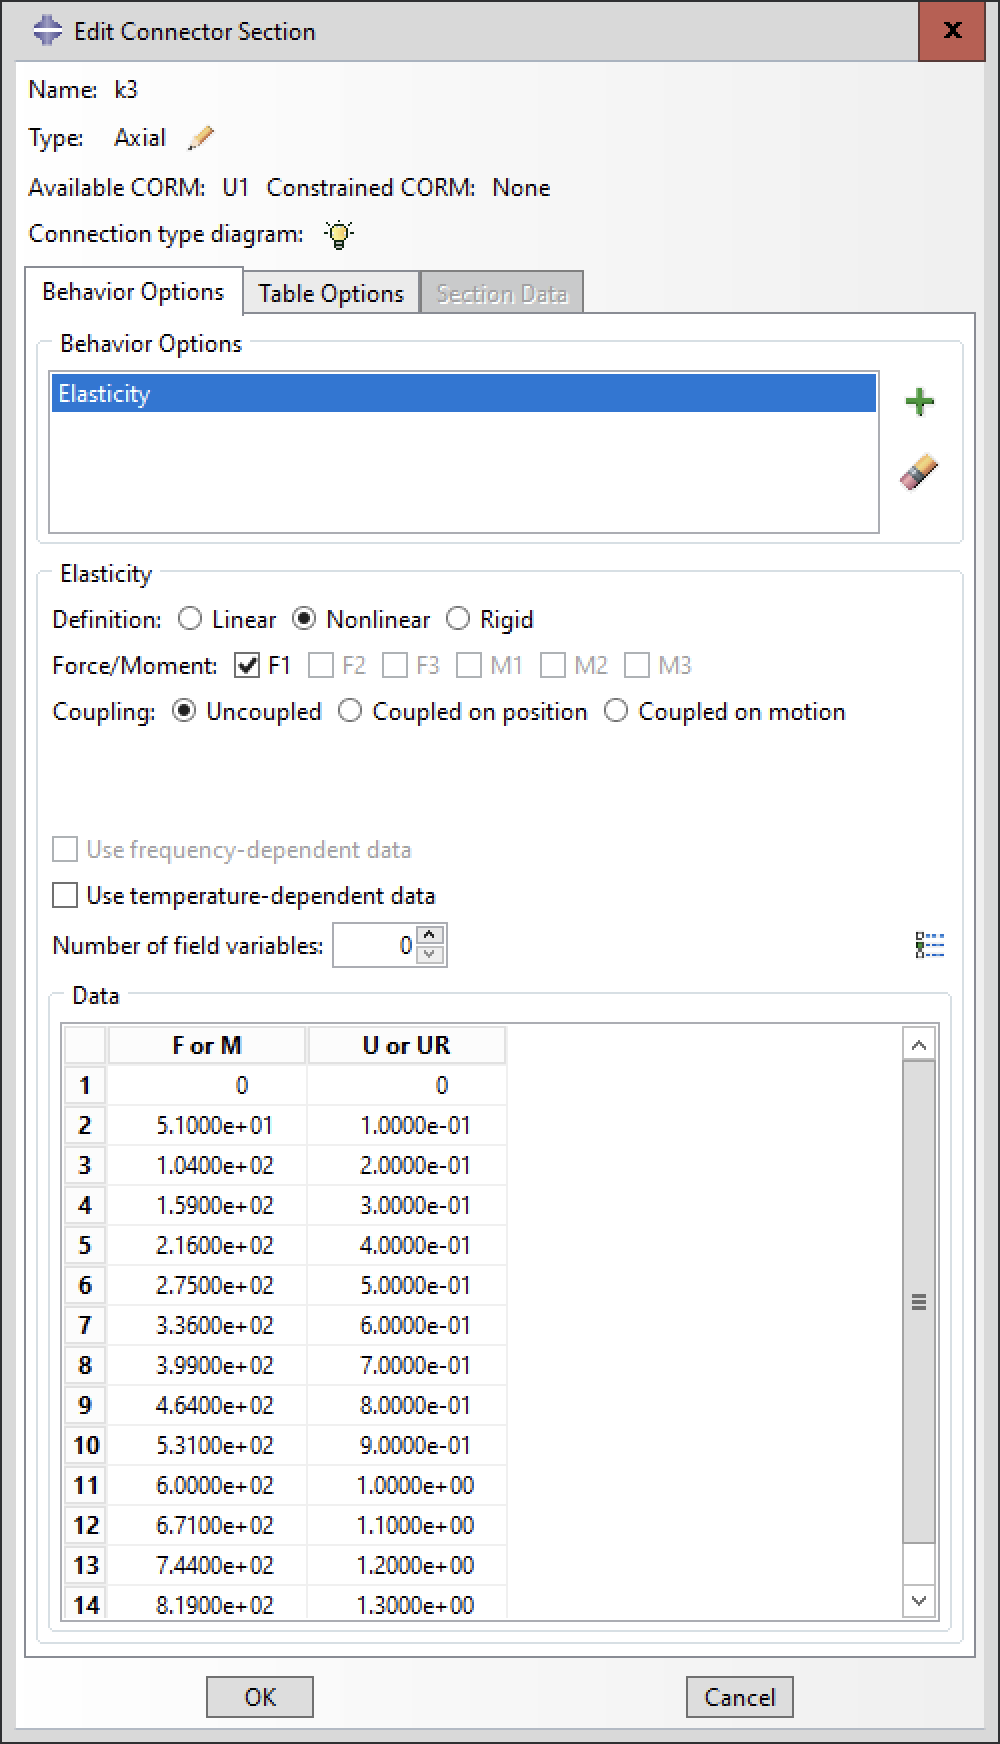
\includegraphics[scale=0.4]{Images/ab1/a9.png}
    }
    \caption{Behavior options of the springs.}
    \label{fig:a89}
\end{figure}

Finally, we associate each spring with its respective mechanical property:
\begin{figure}[H]
    \centering
    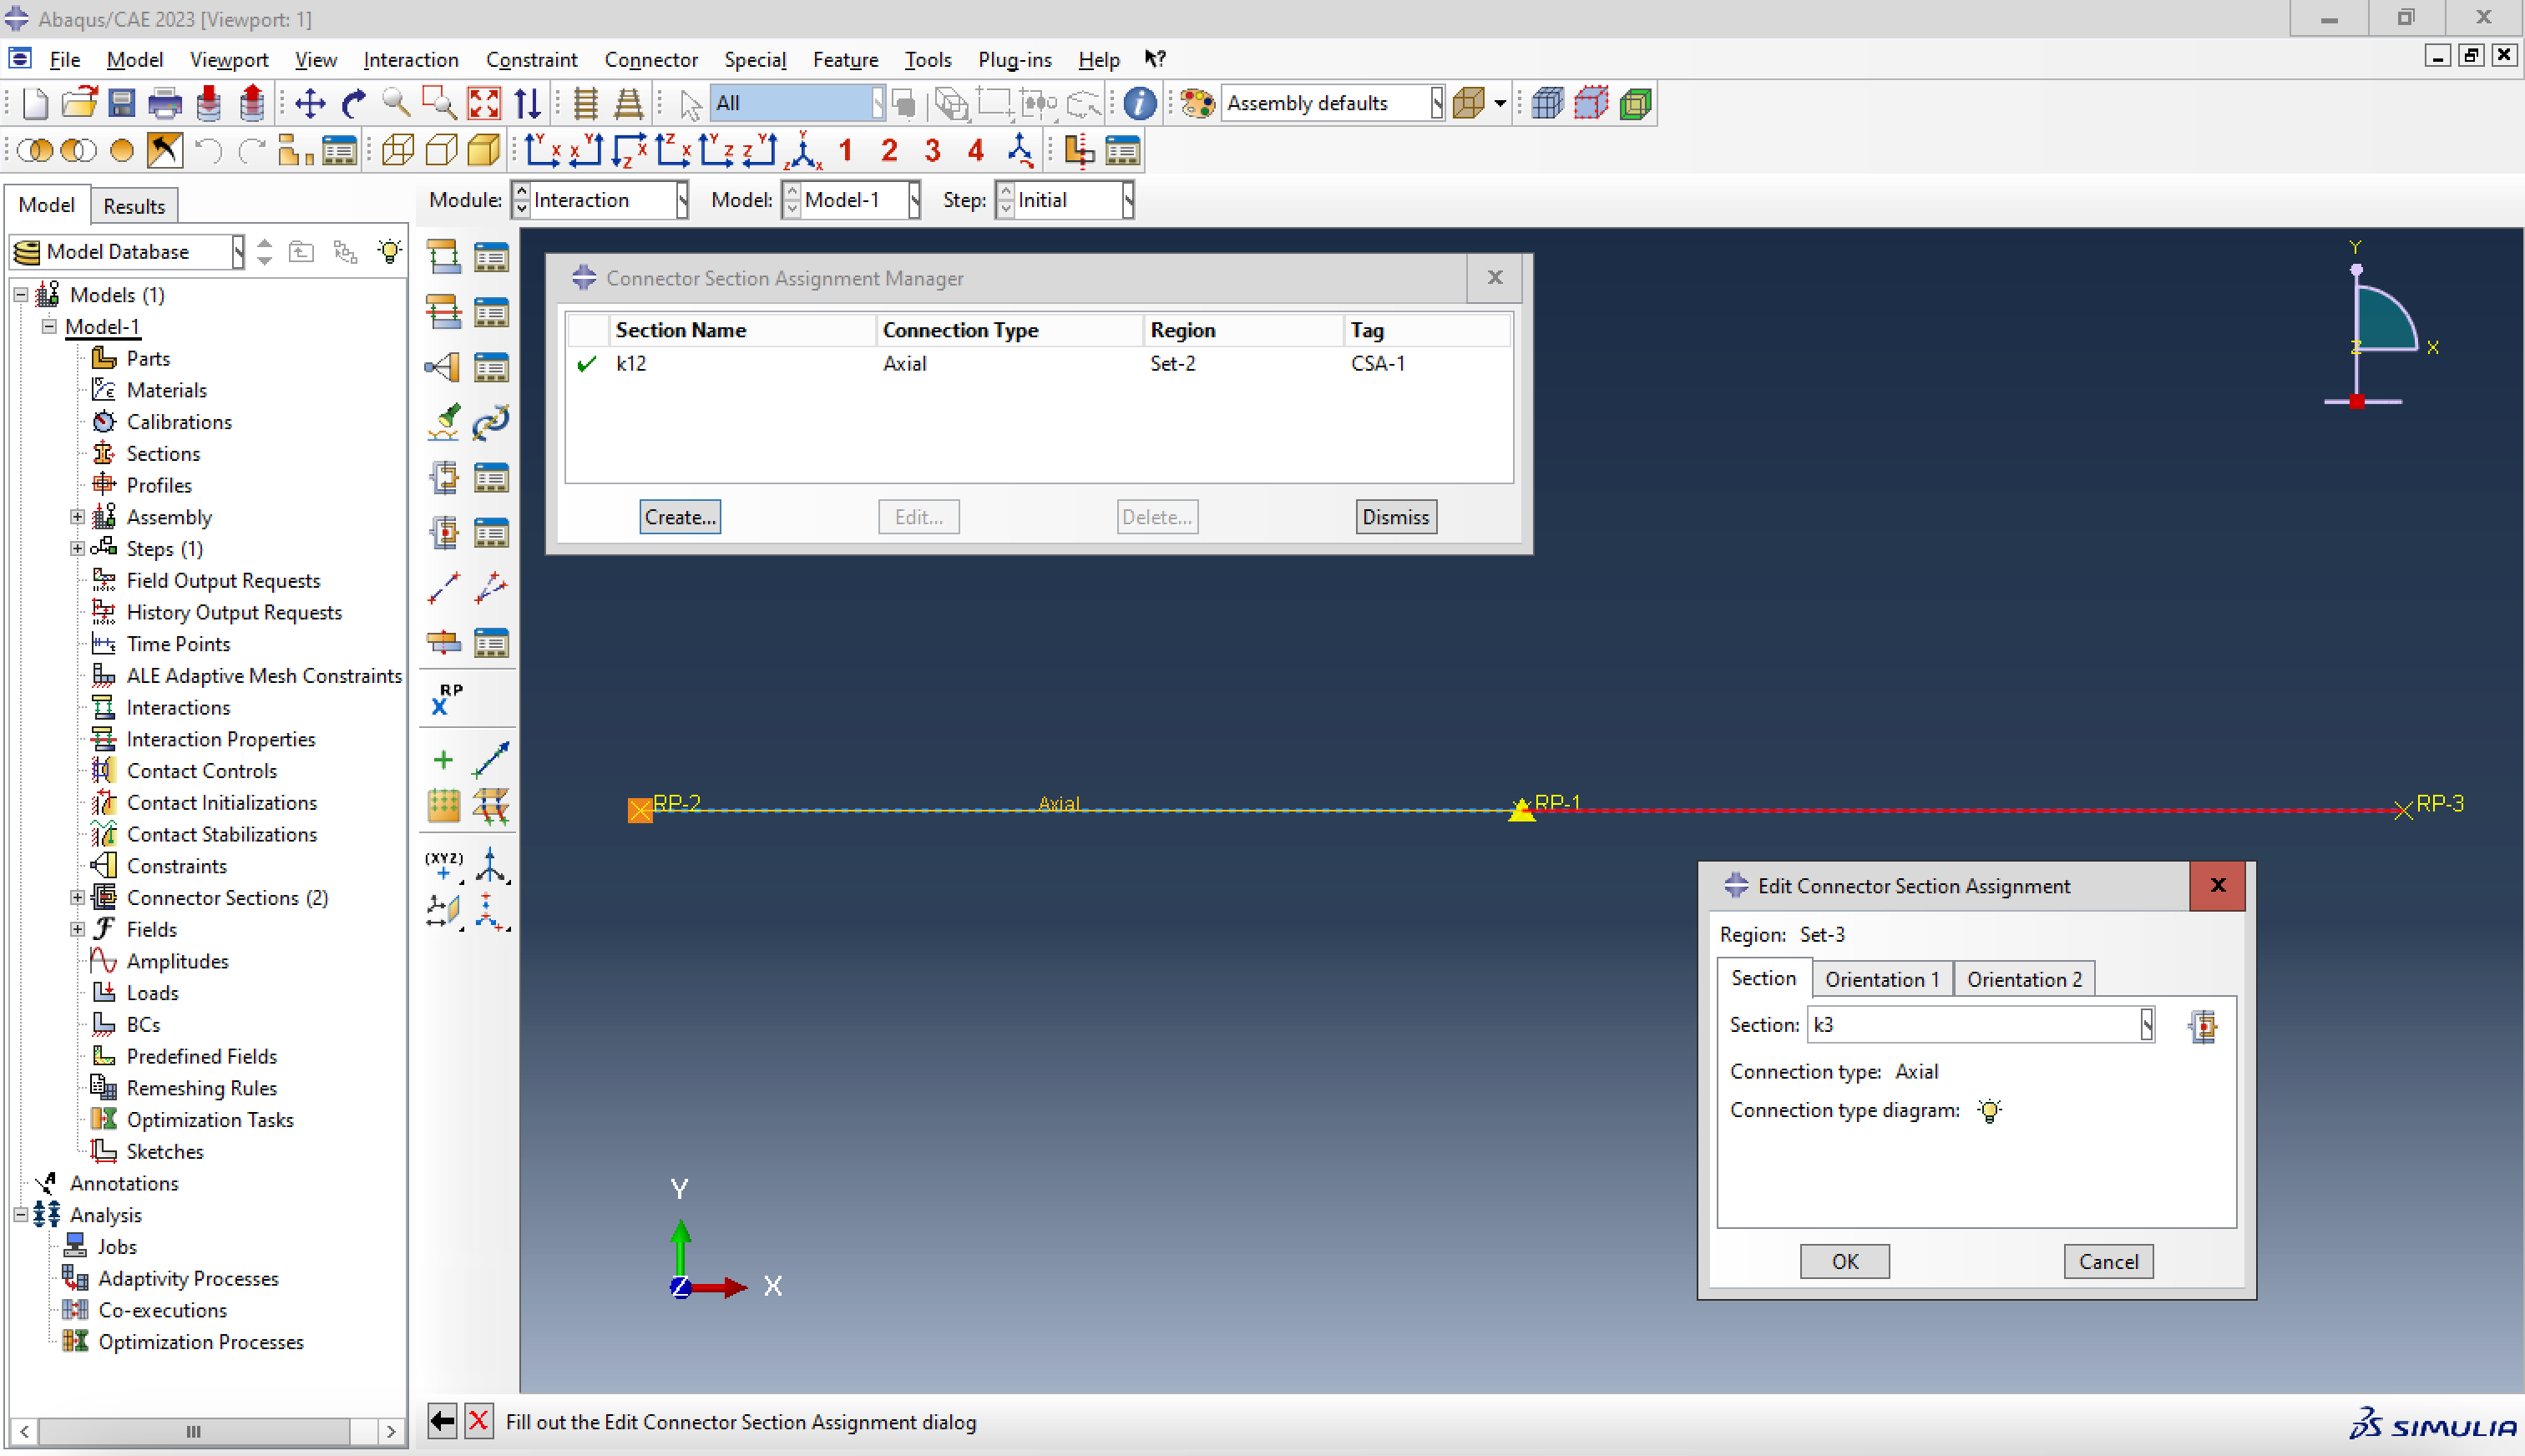
\includegraphics[width=0.9\textwidth]{Images/ab1/a10.png}
    \caption{Connector Section Assignment.}
    \label{fig:a10}
\end{figure}

The final result of this module is shown in Figure~\ref{fig:a11}.
\begin{figure}[H]
    \centering
    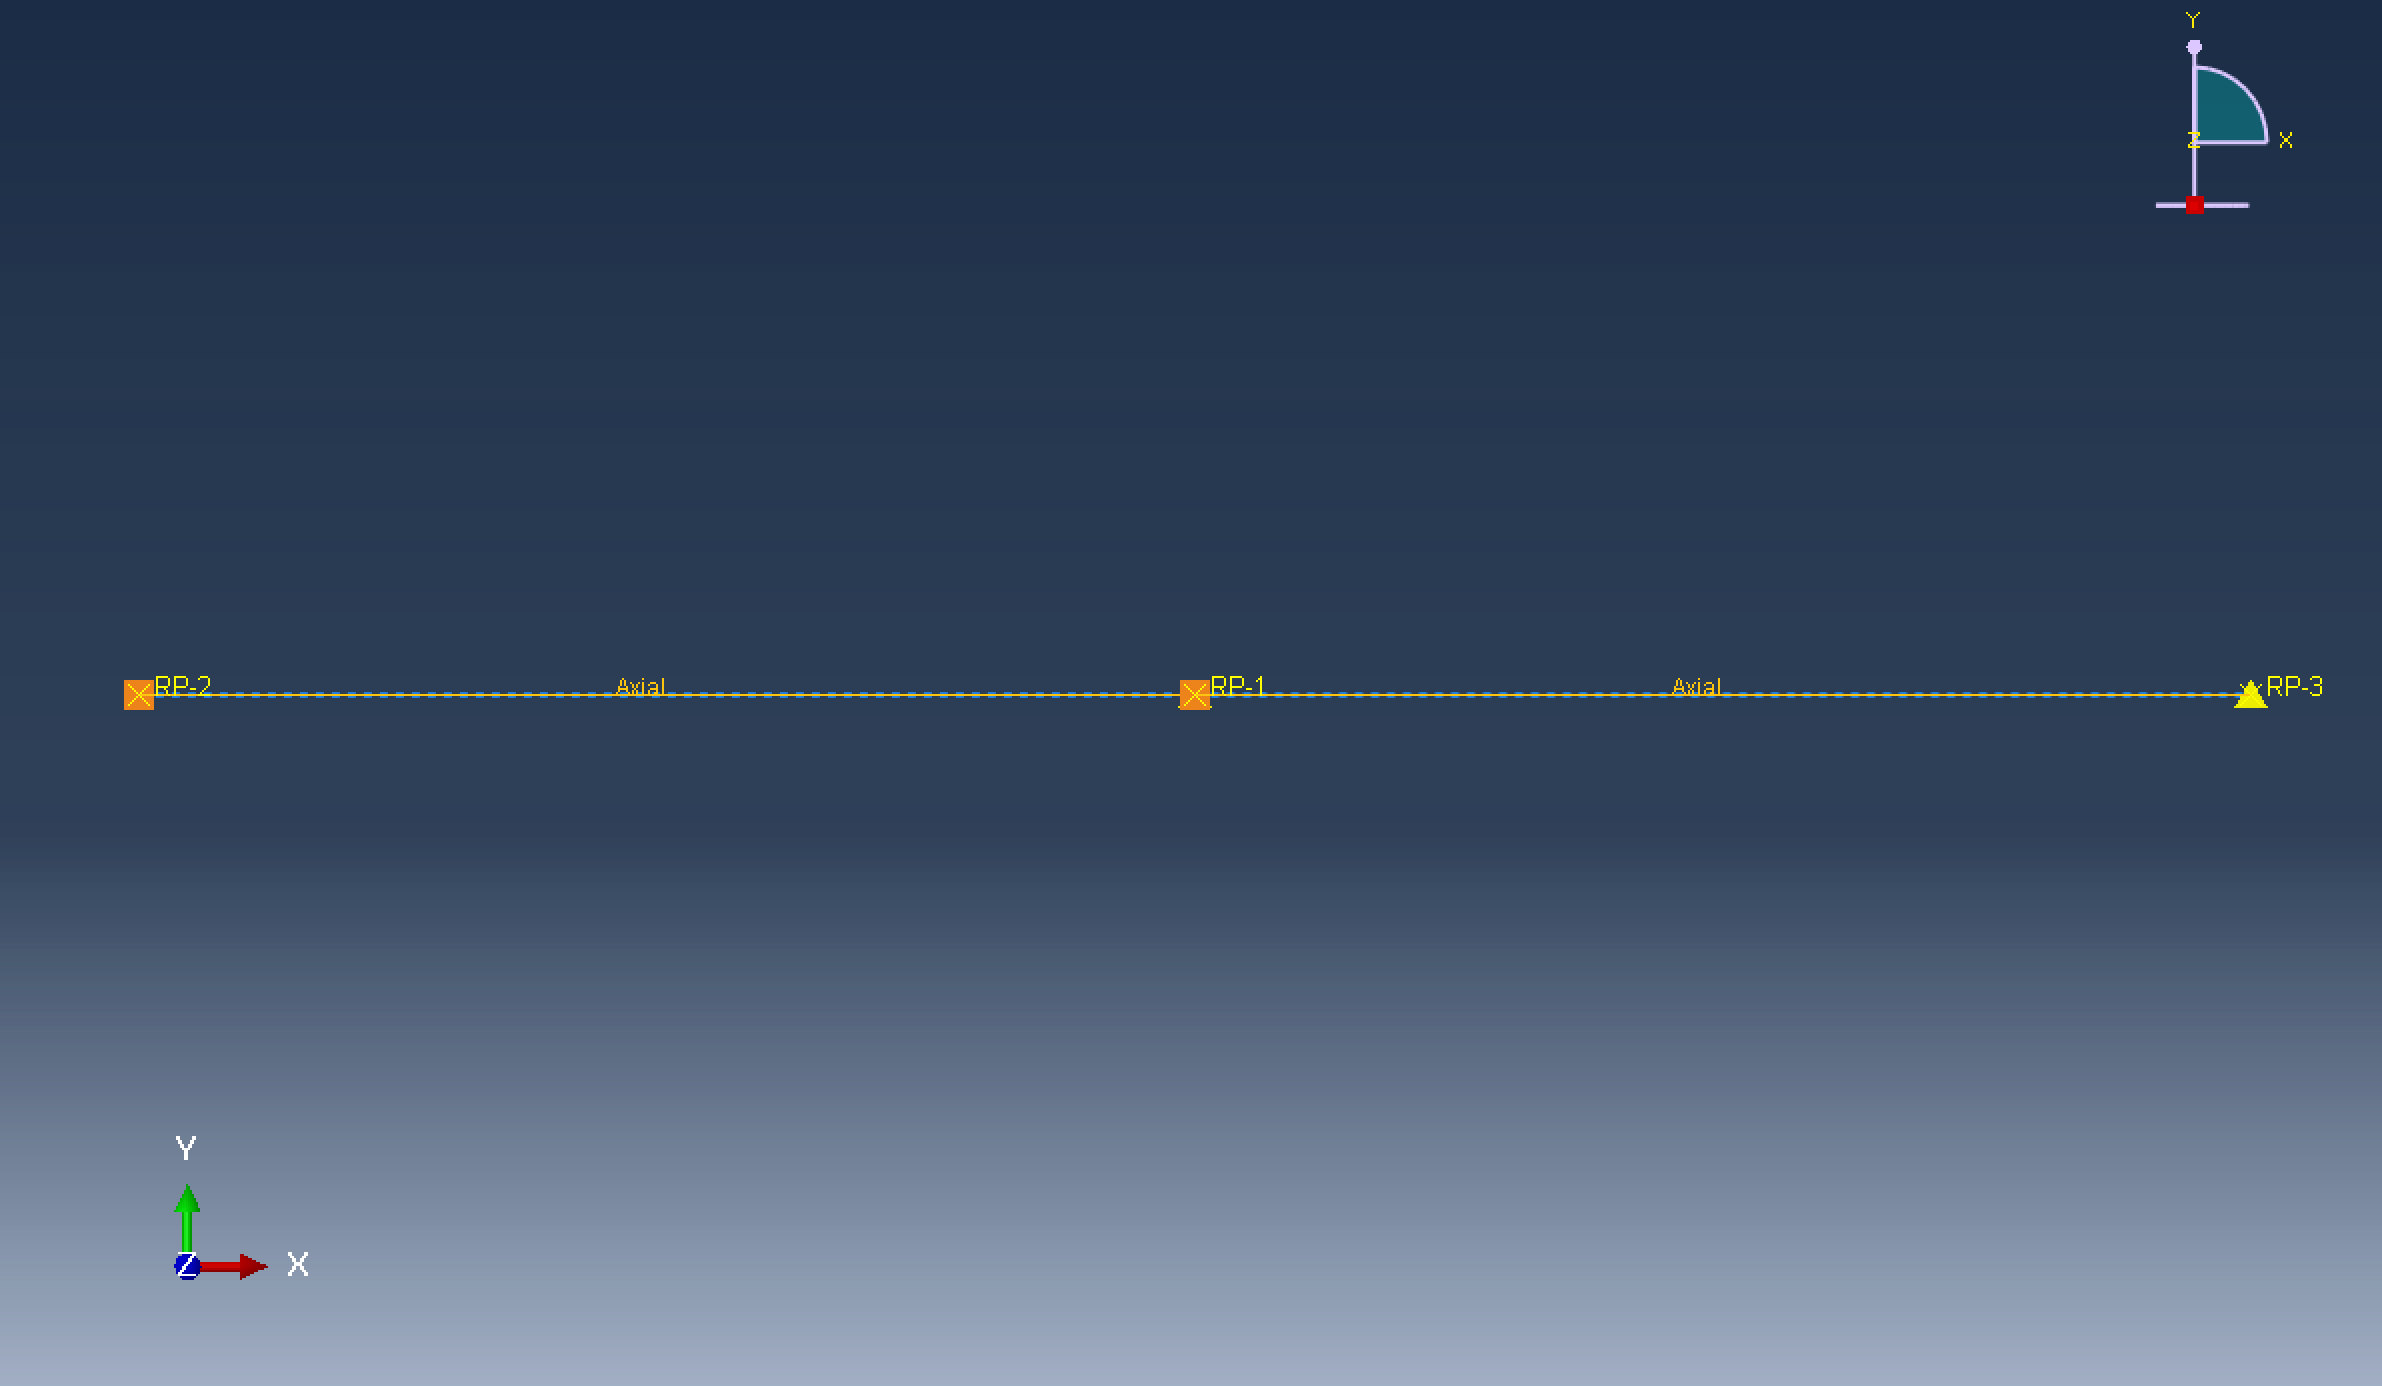
\includegraphics[width=0.9\textwidth]{Images/ab1/a11.png}
    \caption{Final result of Interaction module.}
    \label{fig:a11}
\end{figure} 

\newpage

\subsection{Step module}
\label{step_module1}%

We click on the "Step Manager" button, which looks like Figure~\ref{fig:a12},

\begin{figure}[H]
    \centering
    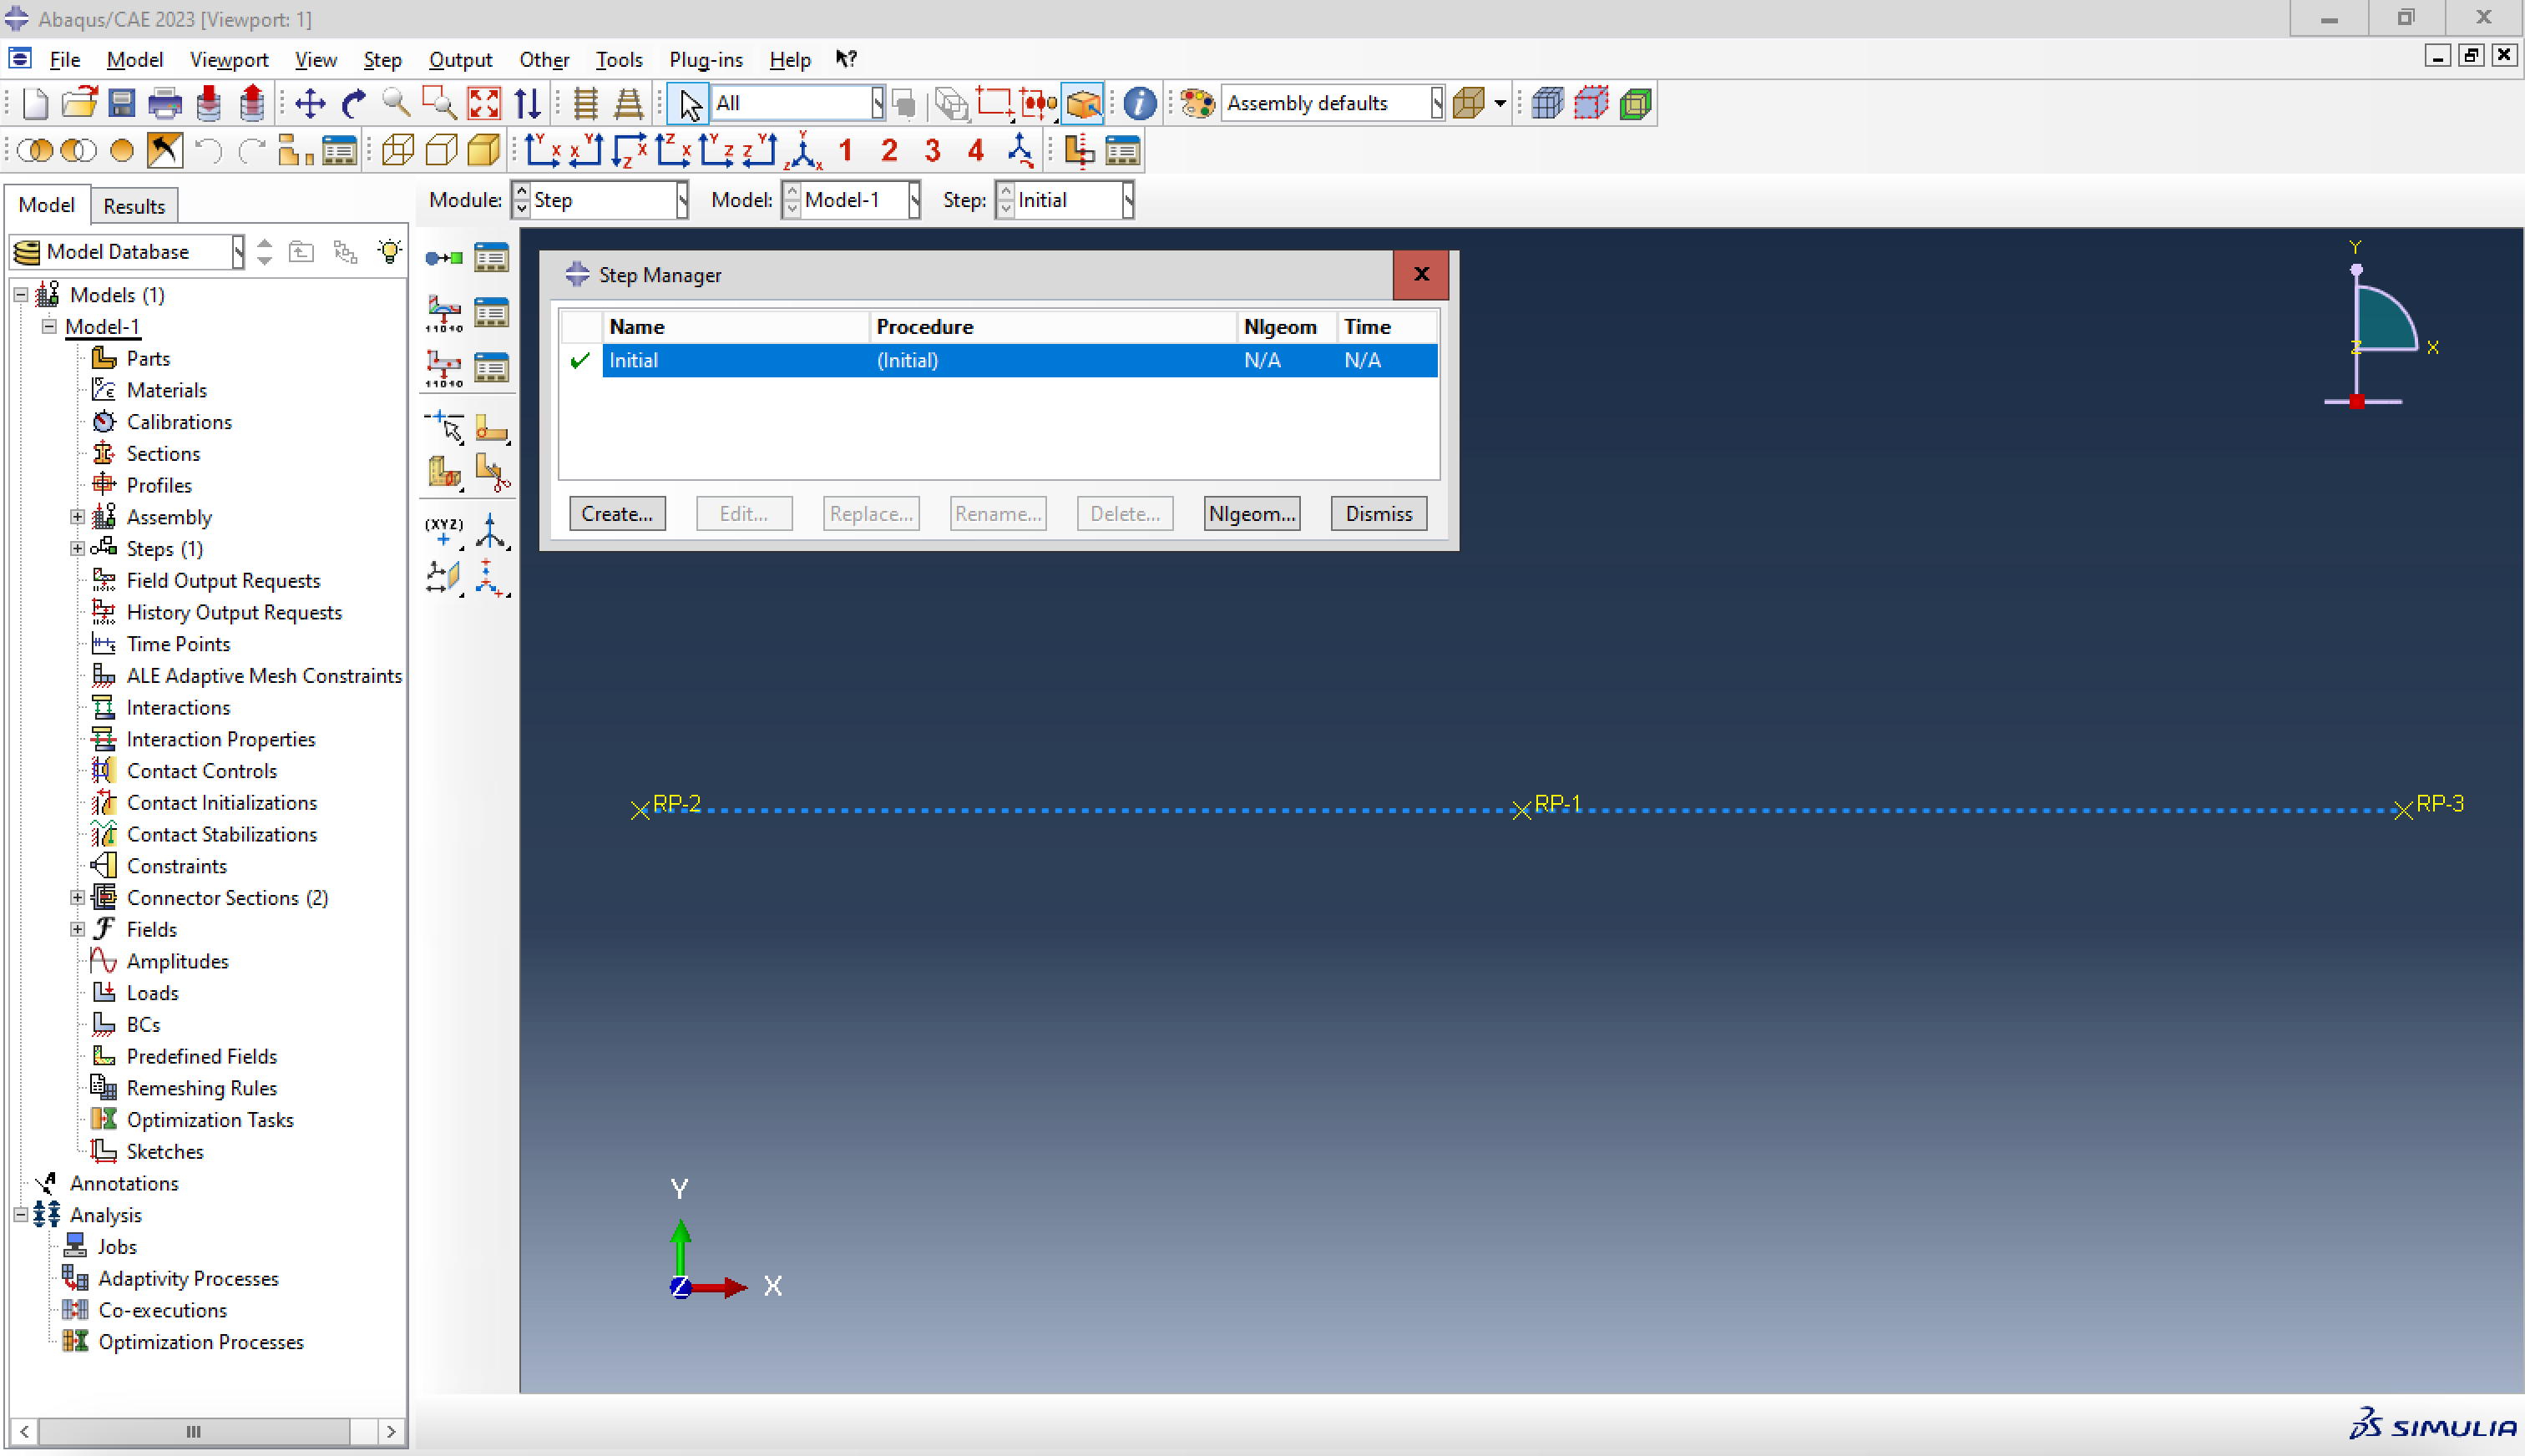
\includegraphics[width=0.9\textwidth]{Images/ab1/a12.png}
    \caption{Step Manager.}
    \label{fig:a12}
\end{figure}

and we create a new step turning on the Nlgeom option (in order to include the nonlinear effects of large displacements):
\begin{figure}[H]
    \centering
    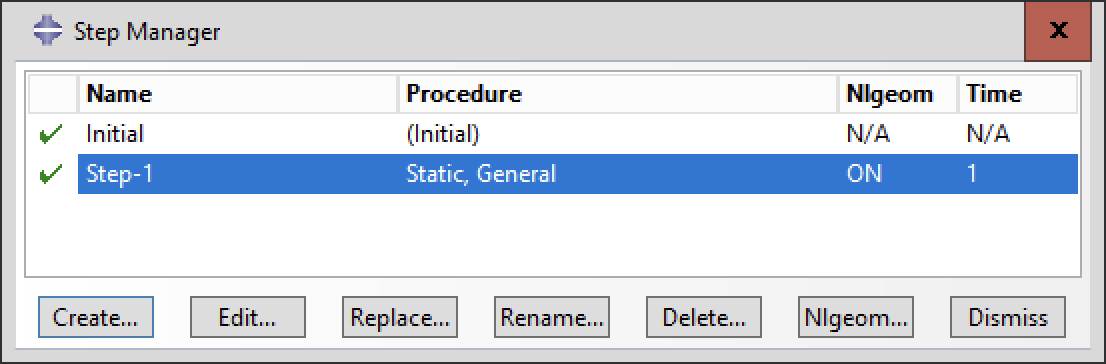
\includegraphics[width=0.4\textwidth]{Images/ab1/a13.png}
    \caption{Final result of Step module.}
    \label{fig:a13}
\end{figure}

\subsection{Load module}
\label{load_module1}%

In this module we first set the boundary conditions of the problem. For the node on the left we want to restrict the vertical, horizontal, and the out-of-plane displacements. Thus, the node on the left has U1, U2 and U3 restricted. Instead, the middle and the right nodes have just U2 and U3 restricted. Figure~\ref{fig:a14151617} shows the setting.

\begin{figure}[H]
    \centering
    \subfloat{
        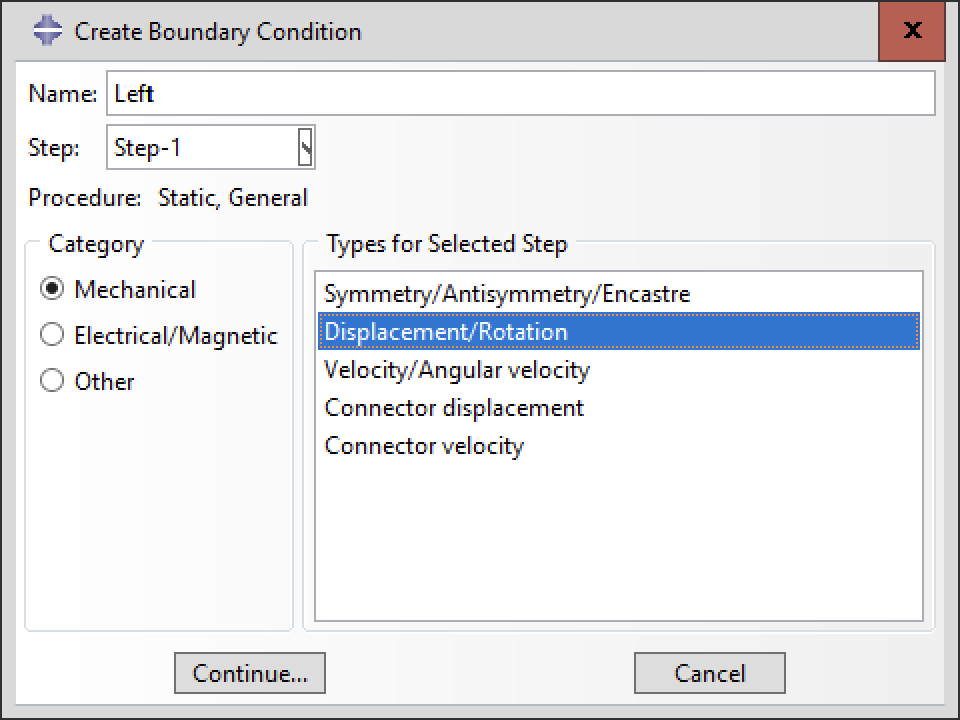
\includegraphics[scale=0.4]{Images/ab1/a14.png}
    }
    \quad
    \subfloat{
        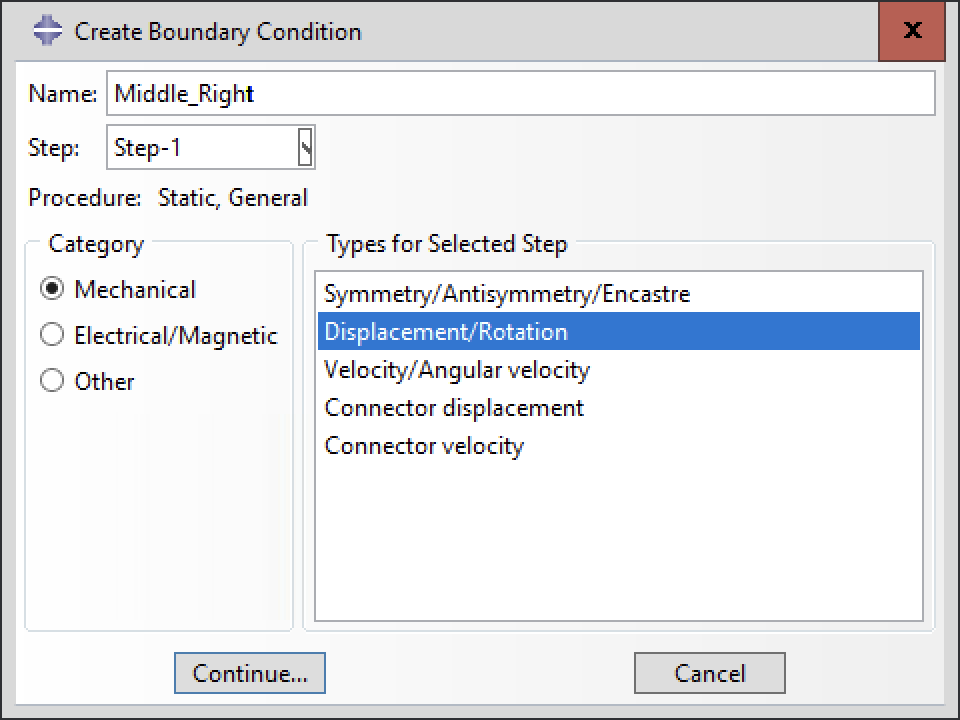
\includegraphics[scale=0.4]{Images/ab1/a16.png}
    }
    \\
    \subfloat{
        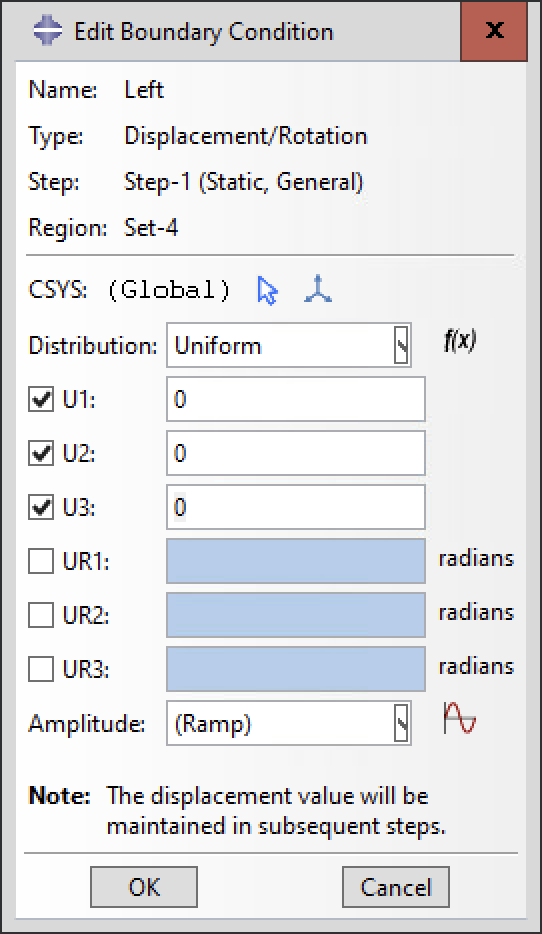
\includegraphics[scale=0.4]{Images/ab1/a15.png}
    }
    \qquad\qquad\qquad
    \subfloat{
        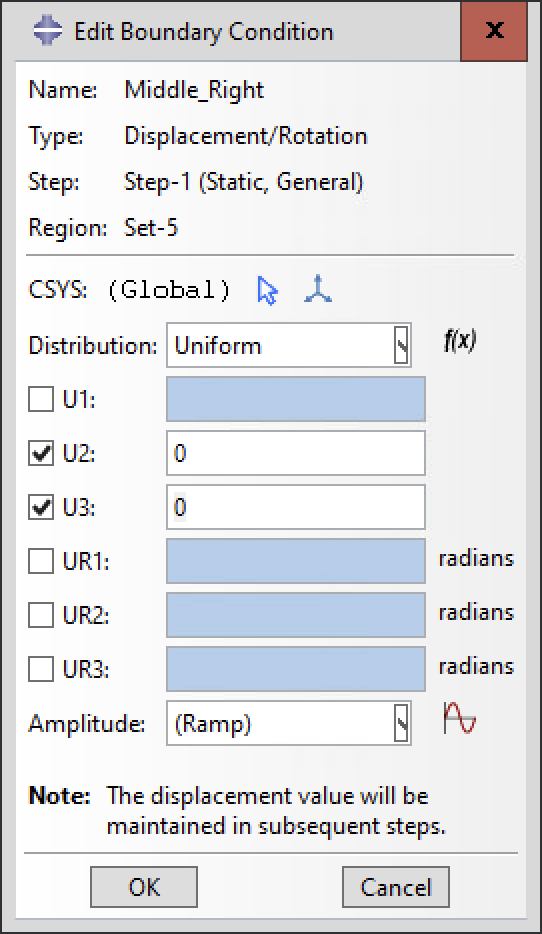
\includegraphics[scale=0.4]{Images/ab1/a17.png}
    }
    \caption{Boundary conditions of the problem.}
    \label{fig:a14151617}
\end{figure}

Then we set a concentrated force of 100 N acting on the right node in the $x$ direction with the "Create Load" symbol:
\begin{figure}[H]
    \centering
    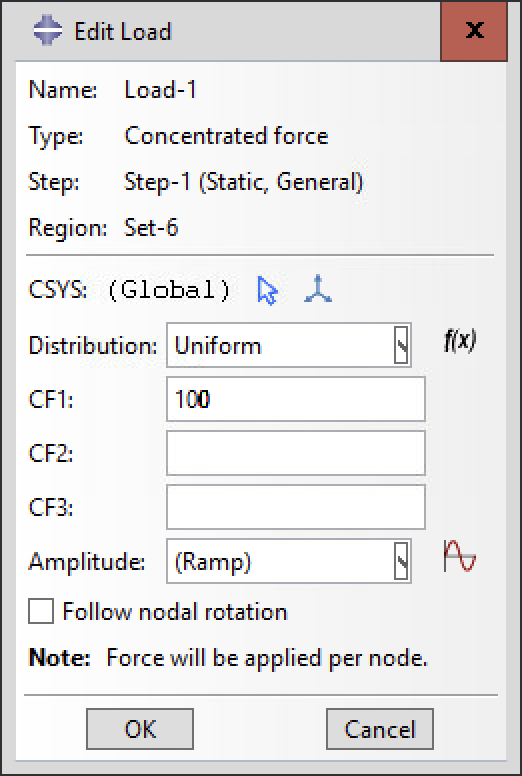
\includegraphics[width=0.25\textwidth]{Images/ab1/a20.png}
    \caption{Load options.}
    \label{fig:a20}
\end{figure}

\newpage

Here there is the result:
\begin{figure}[H]
    \centering
    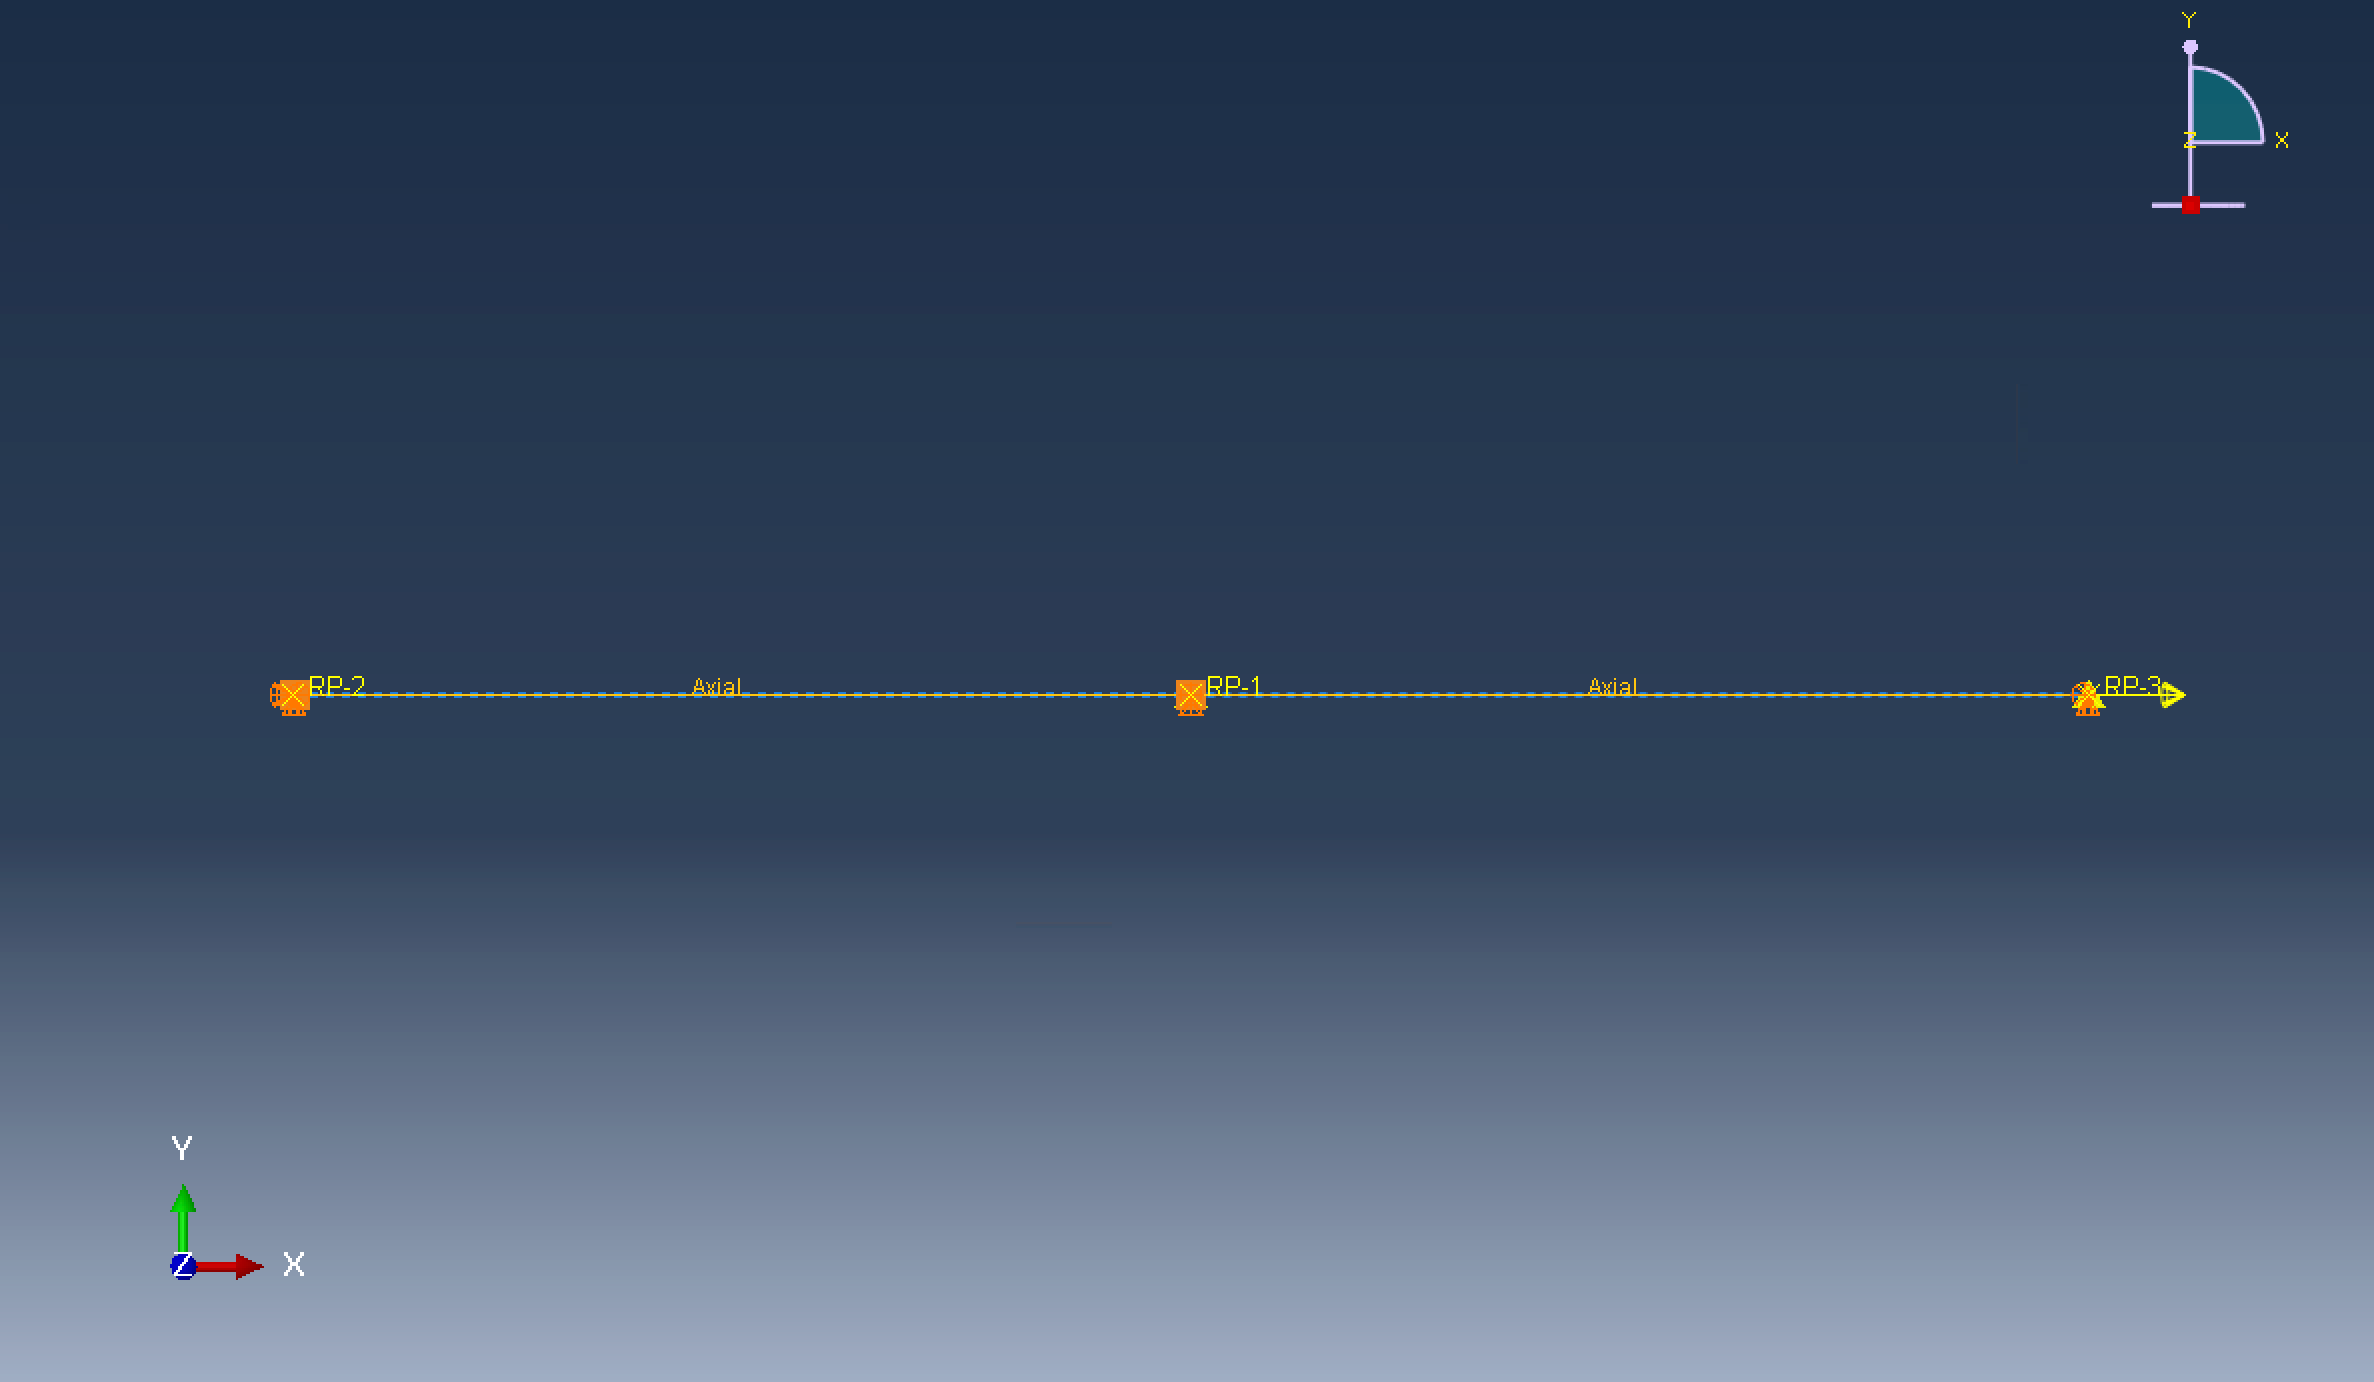
\includegraphics[width=0.9\textwidth]{Images/ab1/a21.png}
    \caption{Final result of Load module.}
    \label{fig:a21}
\end{figure}

\subsection{Job module}
\label{job_module1}%

We create a standard job in the "Job Manager" and we submit it:
\begin{figure}[H]
    \centering
    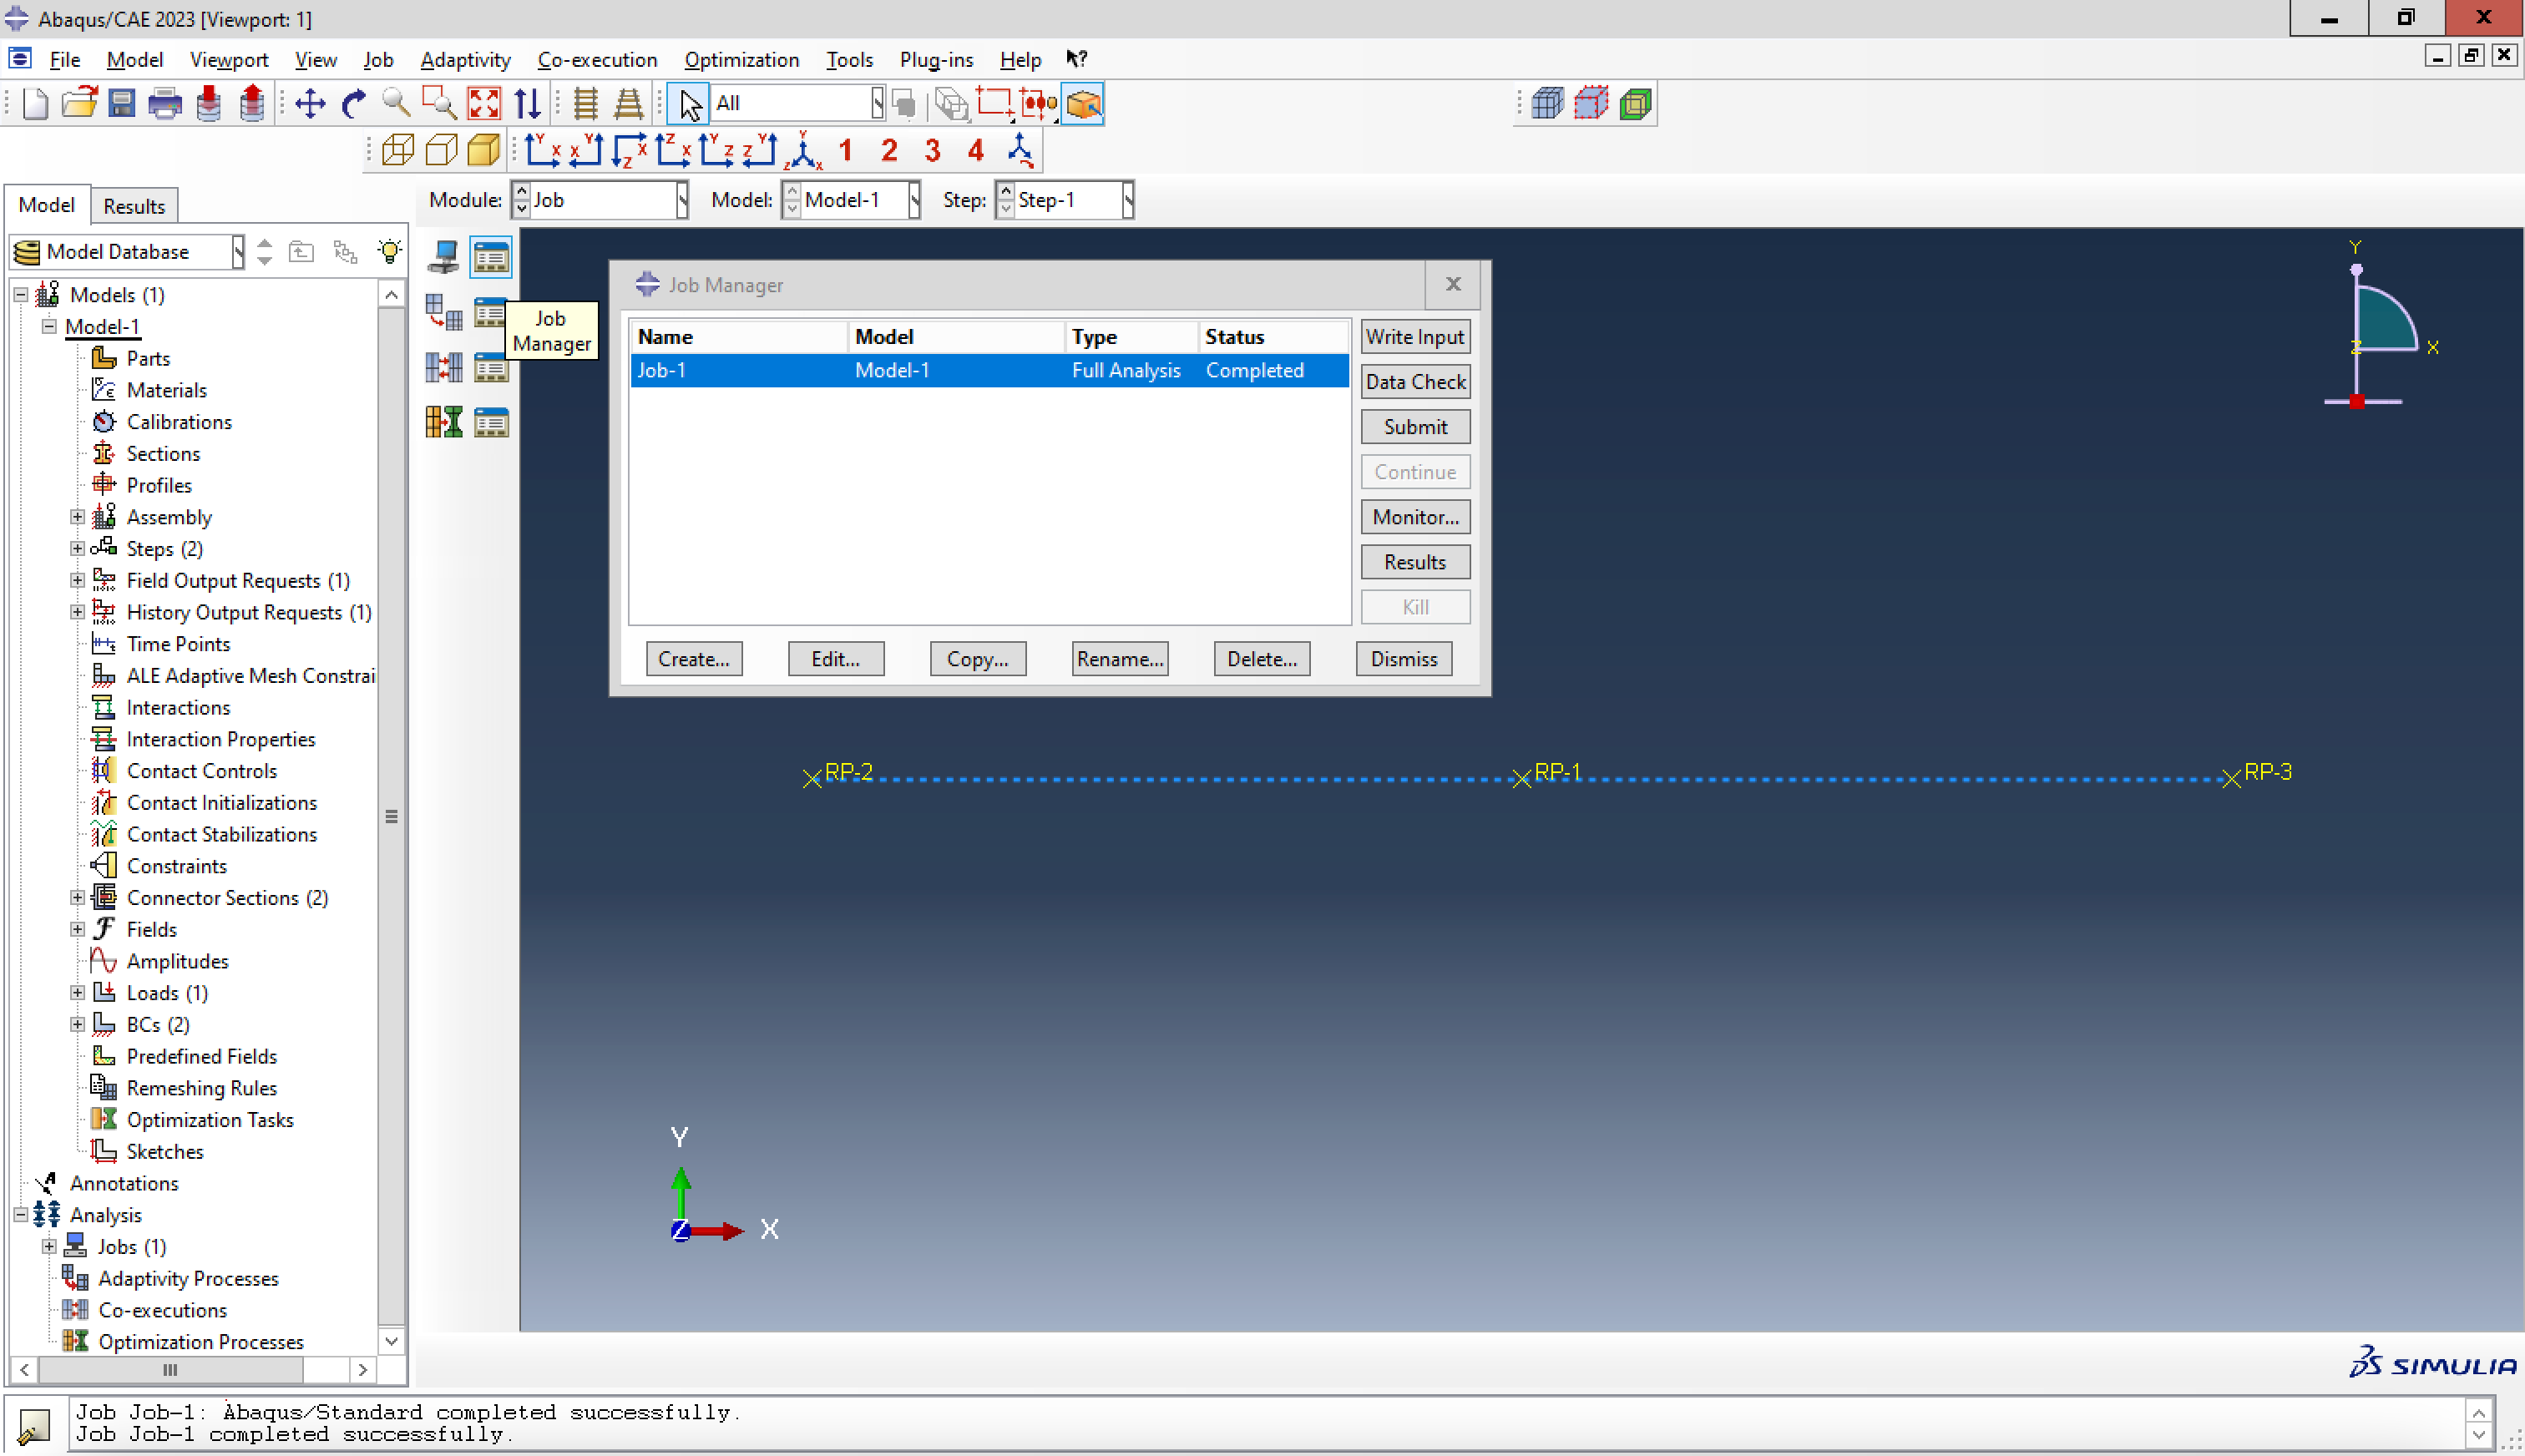
\includegraphics[width=0.9\textwidth]{Images/ab1/a23.png}
    \caption{Final result of Job module.}
    \label{fig:a23}
\end{figure}

\newpage

\subsection{Visualization module}
\label{visualization_module1}%

First, we enable the connectors view in the ODB Display Options, as in Figure~\ref{fig:a24}
\begin{figure}[H]
    \centering
    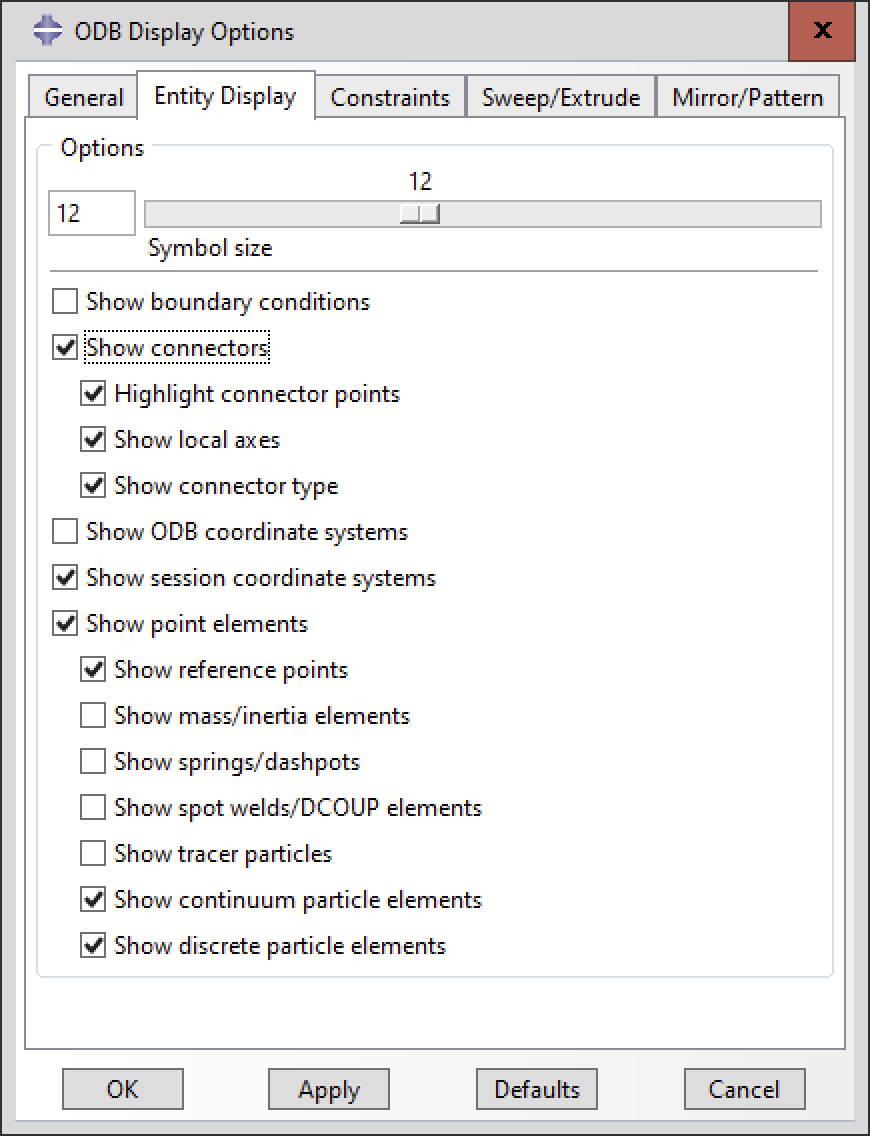
\includegraphics[width=0.3\textwidth]{Images/ab1/a24.png}
    \caption{View ODB Display Options.}
    \label{fig:a24}
\end{figure}

Here is the result we obtained:
\begin{figure}[H]
    \centering
    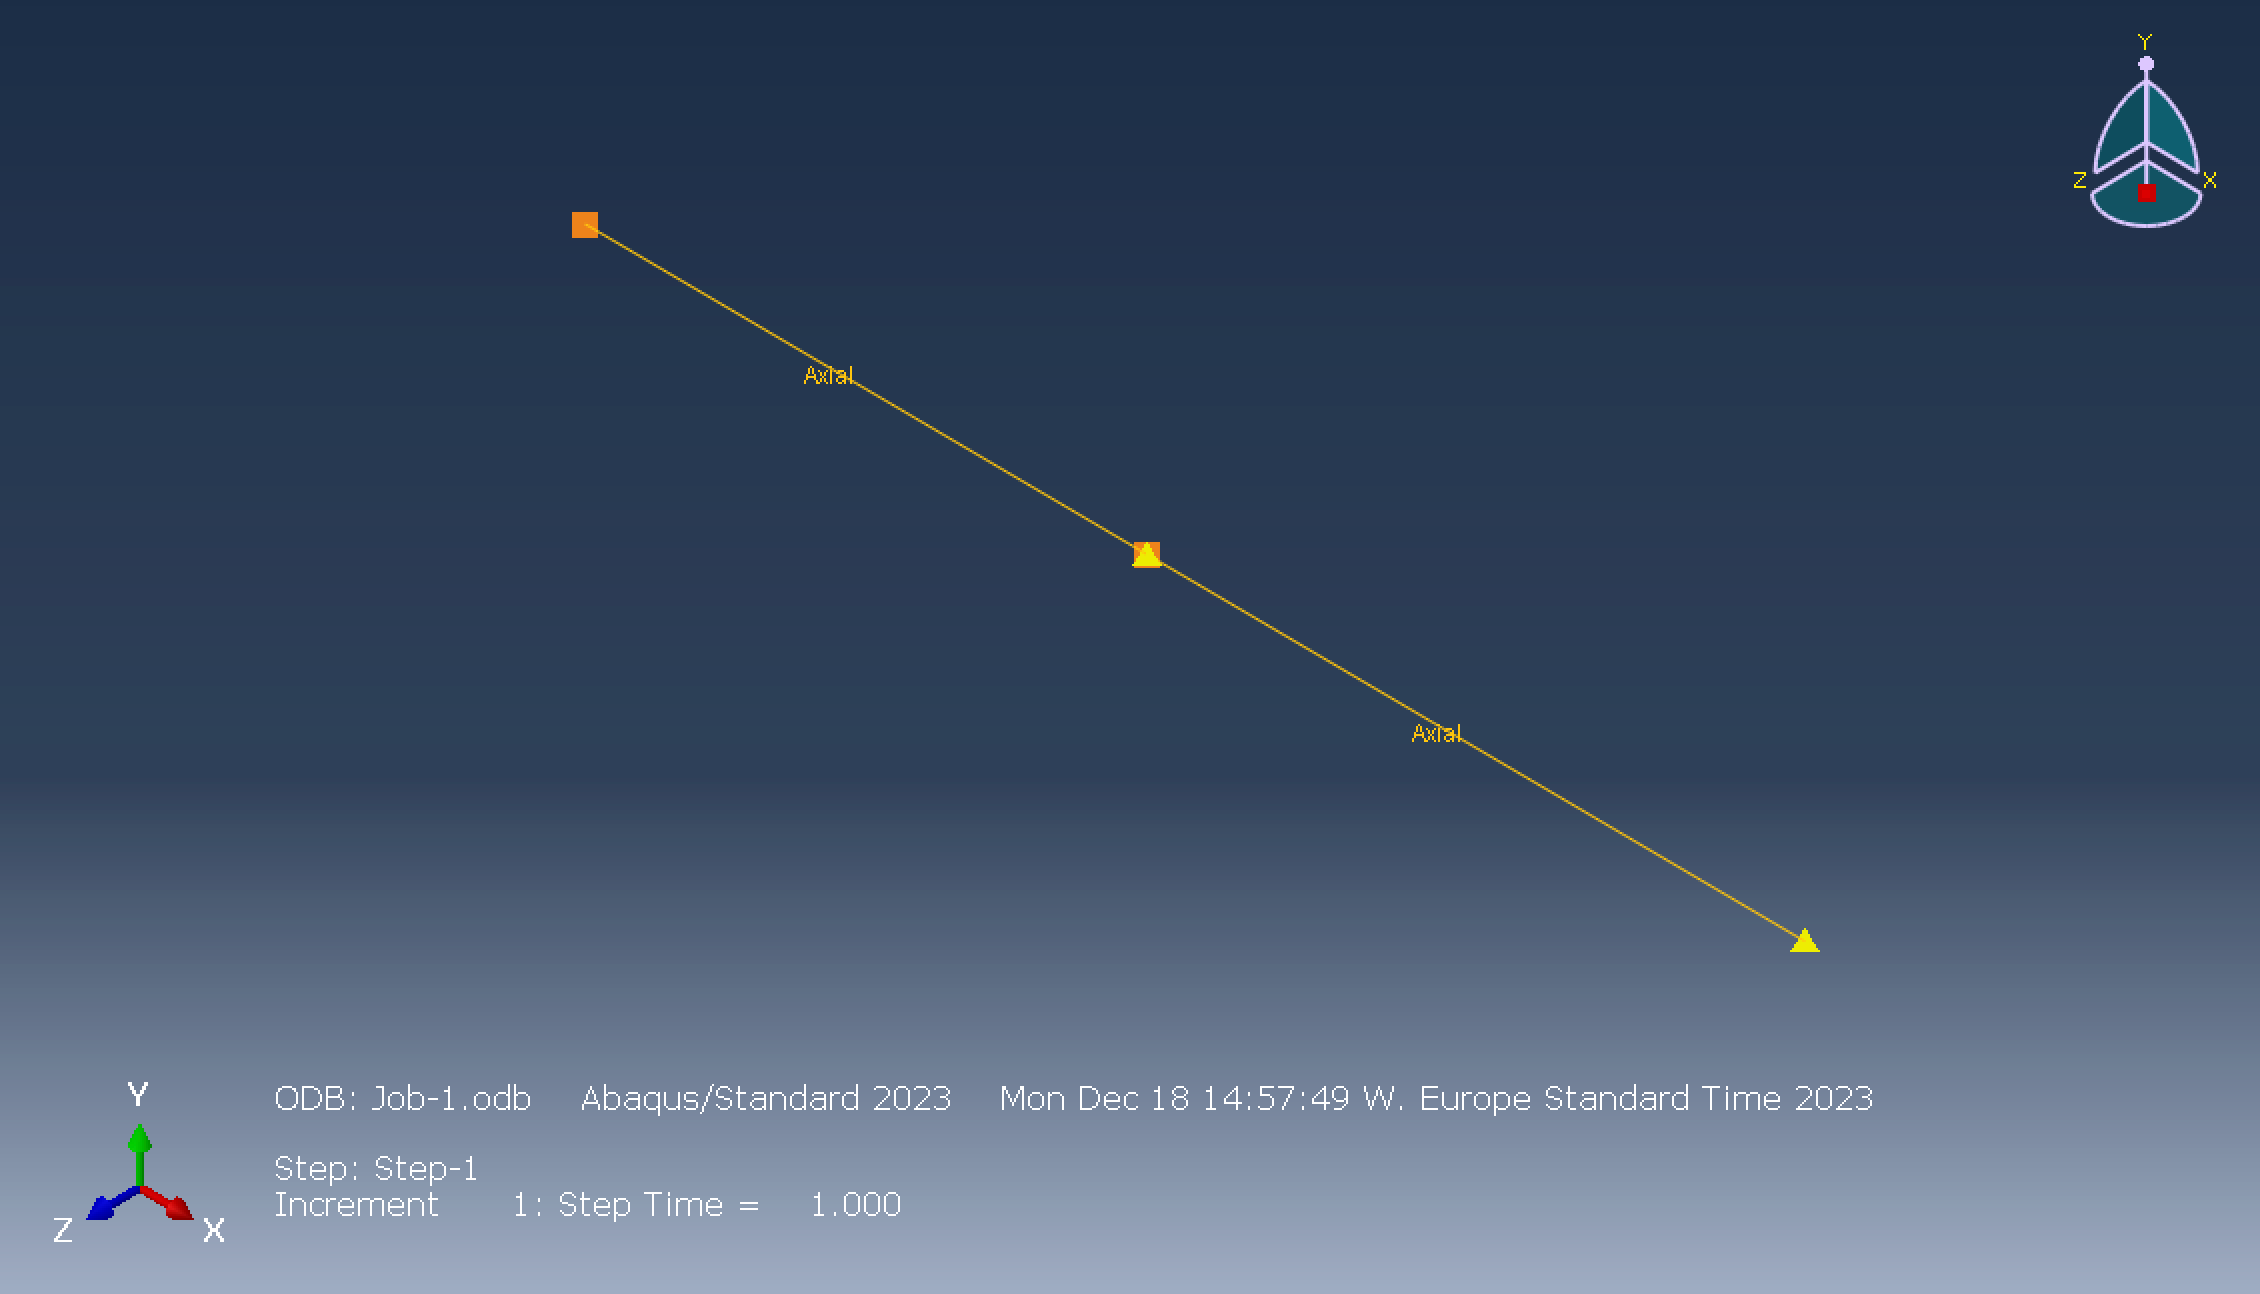
\includegraphics[width=0.9\textwidth]{Images/ab1/a25.png}
    \caption{Final result.}
    \label{fig:a25}
\end{figure}

\newpage

We can explain U1 thanks to Figure~\ref{fig:a26}.

\begin{figure}[H]
    \centering
    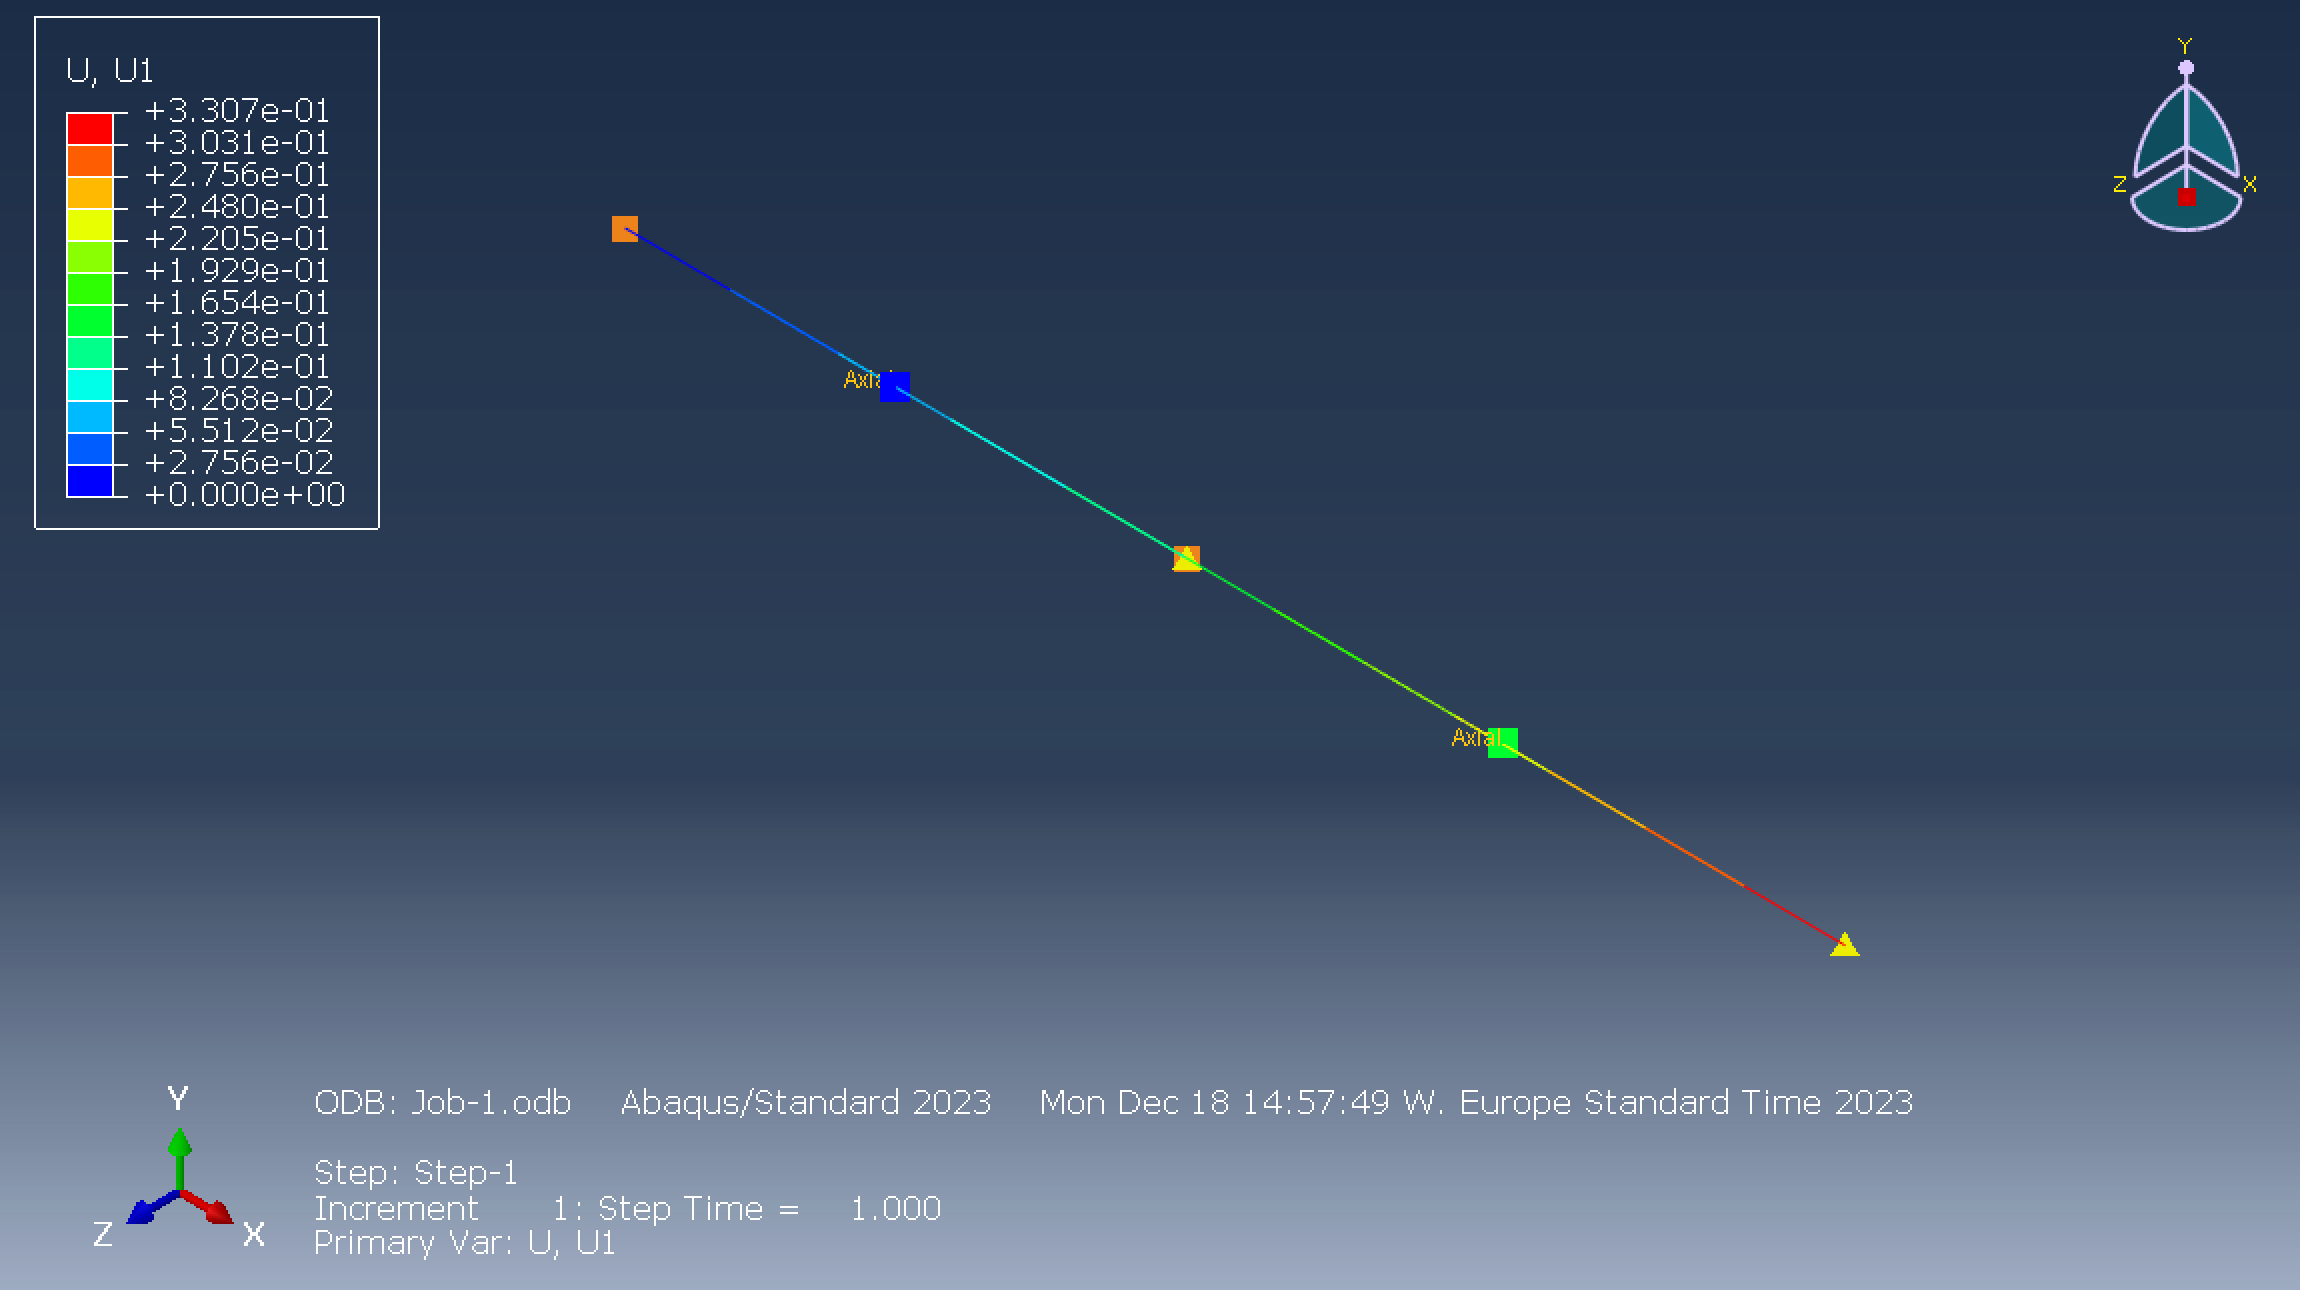
\includegraphics[width=0.9\textwidth]{Images/ab1/a26.png}
    \caption{Final result in term of U1.}
    \label{fig:a26}
\end{figure}

To be more precise, we proceed by clicking on the "Create XY Data" symbol and then we select the spatial displacement of U1 of the middle and right nodes (the ones we are interested in):
\begin{figure}[H]
    \centering
    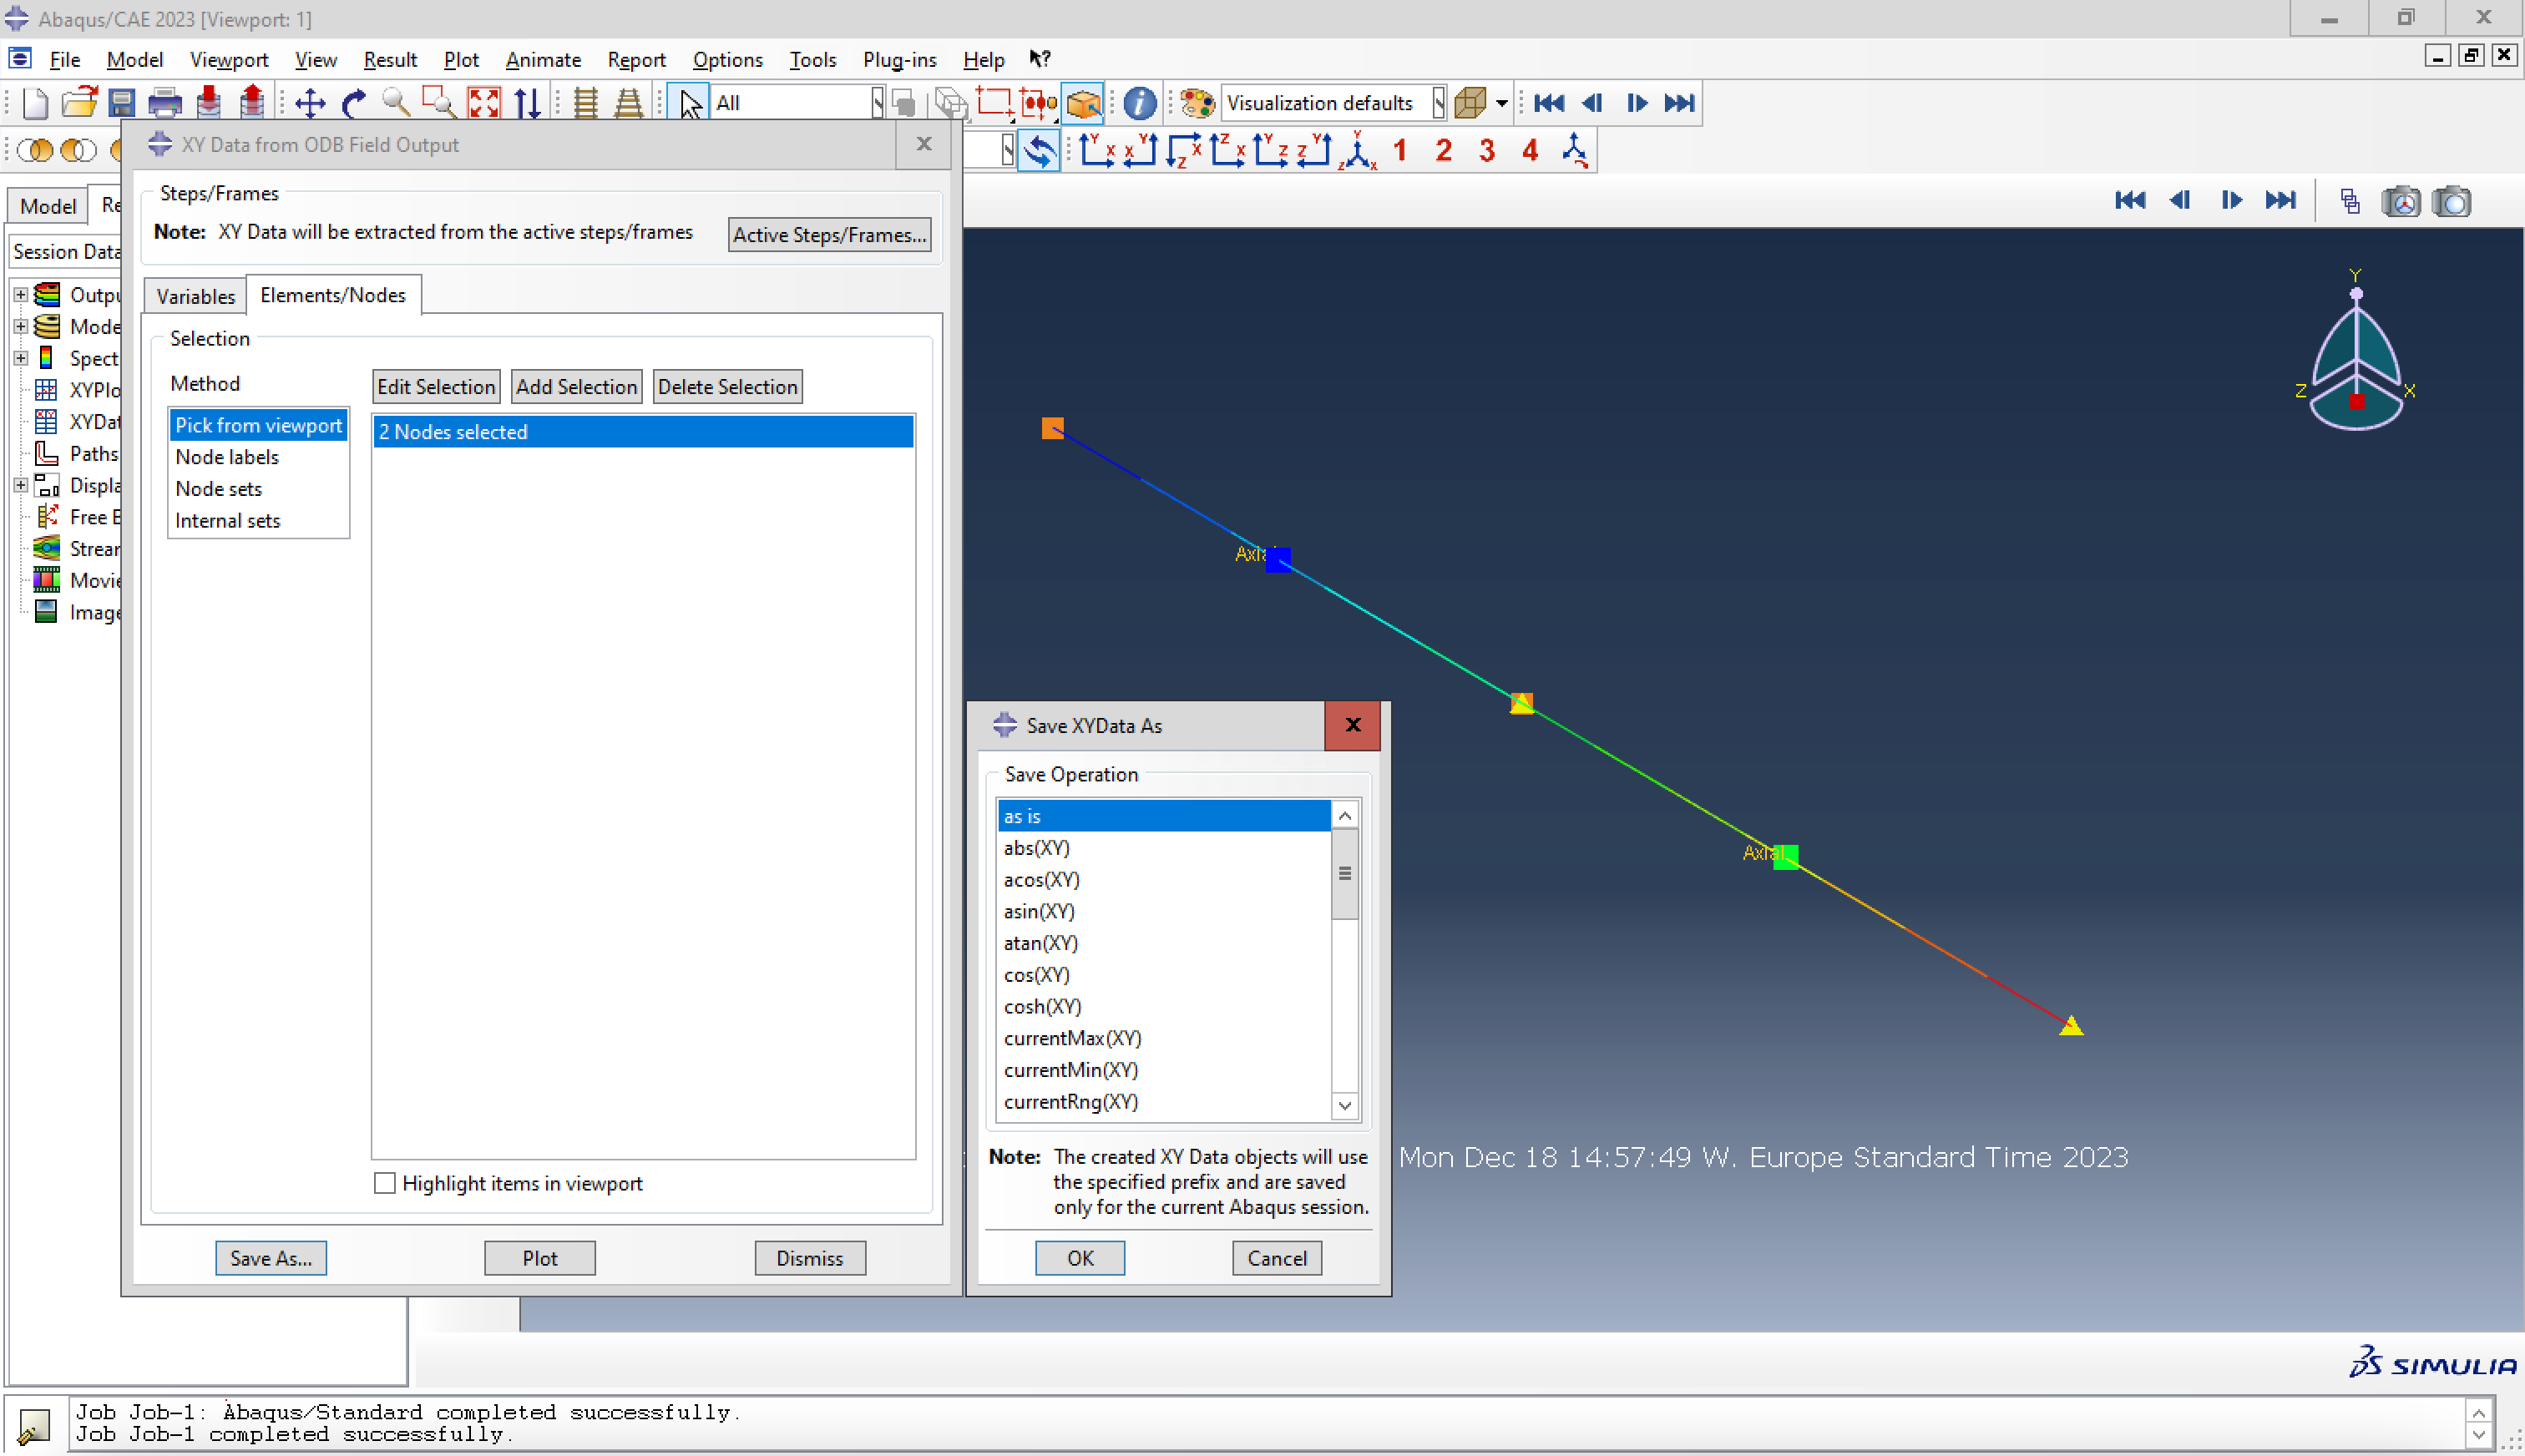
\includegraphics[width=0.9\textwidth]{Images/ab1/a29.png}
    \caption{XY Data from ODB Field Output.}
    \label{fig:a29}
\end{figure}

\newpage

Finally, by going into the \emph{edit} option of each displacement we can check the numerical result for each selected node:
\begin{figure}[H]
    \centering
    \subfloat{
        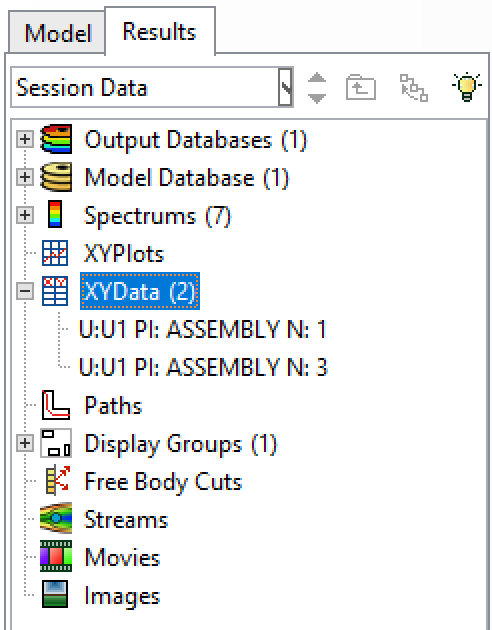
\includegraphics[scale=0.5]{Images/ab1/a30.png}
    }
    \quad
    \subfloat{
        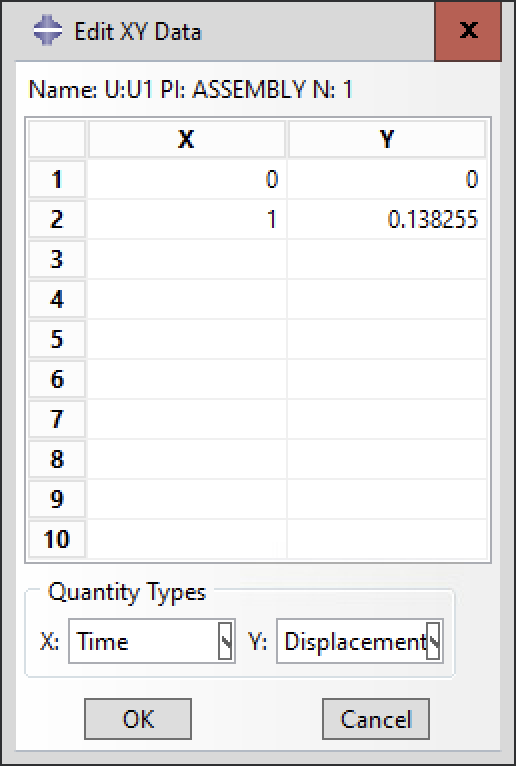
\includegraphics[scale=0.4]{Images/ab1/a31.png}
    }
    \quad
    \subfloat{
        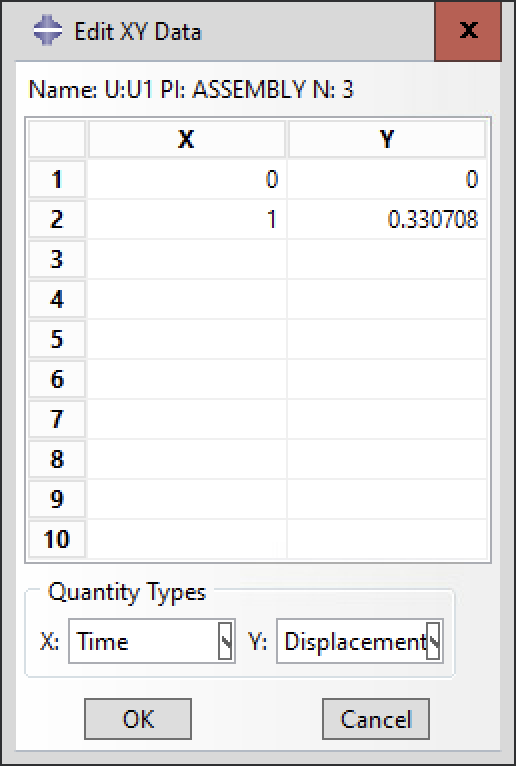
\includegraphics[scale=0.4]{Images/ab1/a32.png}
    }    
    \caption{Numerical results with Abaqus.}
    \label{fig:a303132}
\end{figure}

\section{Comparison between MATLAB and Abaqus}
\label{sec:comparison1}%

Now we compare the values previously obtained with MATLAB and Abaqus.

\begin{table}[H]
    %\caption*{\textbf{Title of Table (optional)}}
    \centering 
    \begin{tabular}{lcccc}
    \hline
    \rowcolor{bluepoli!40} % comment this line to remove the color
    Quantity & Symbol & MATLAB & Abaqus & UoM \\
    \hline
    Horizontal middle displacement & $u_1$ & 0.13873 & 0.138255 & mm \\
    Horizontal right displacement & $u_2$ & 0.33132 & 0.330708 & mm \\
    \hline
    \end{tabular}
    \\[10pt]
    \caption{MATLAB and Abaqus results.}
    \label{table:alpha_beta}
\end{table}

In conclusion, the analysis of the results obtained through simulation in MATLAB and Abaqus confirms the accuracy of the proposed model, highlighting a congruent agreement between the two software and the adopted theoretical methodology.